\documentclass{article}

\PassOptionsToPackage{numbers,sort&compress}{natbib}
\usepackage[preprint]{neurips_2026}

\usepackage[utf8]{inputenc}
\usepackage[T1]{fontenc}
\usepackage{hyperref}
\usepackage{url}
\usepackage{booktabs}
\usepackage{graphicx}
\usepackage{amsmath,amssymb,amsfonts,amsthm}
\usepackage{multirow}
\usepackage{enumitem}
\usepackage{microtype}
\usepackage{xcolor}
\usepackage[normalem]{ulem}

\newcommand{\pier}[1]{{\color{red}Pier: #1}}

\newtheorem{assumption}{Assumption}
\newtheorem{definition}{Definition}
\newtheorem{theorem}{Theorem}
\newtheorem{lemma}{Lemma}
\newtheorem{proposition}{Proposition}
\newtheorem{corollary}{Corollary}
\newtheorem{remark}{Remark}

\newcounter{algorithm}
\newenvironment{algorithm}[1][]{%
  \refstepcounter{algorithm}%
  \par\medskip
  \noindent\textbf{Algorithm~\thealgorithm}%
  \if\relax\detokenize{#1}\relax\else\ \normalfont(#1).\fi%
  \par\vspace{0.45em}%
  \normalfont\small
}{%
  \par\medskip
}

\DeclareMathOperator*{\argmin}{arg\,min}
\DeclareMathOperator*{\argmax}{arg\,max}
\DeclareMathOperator{\KL}{KL}
\DeclareMathOperator{\MI}{I}
\DeclareMathOperator{\Hent}{H}
\DeclareMathOperator{\Occ}{Occ}

\newcommand{\cA}{\mathcal{A}}
\newcommand{\cBdiag}{\mathcal{B}_{\mathrm{diag}}}
\newcommand{\cD}{\mathcal{D}}
\newcommand{\cF}{\mathcal{F}}
\newcommand{\cM}{\mathcal{M}}
\newcommand{\cS}{\mathcal{S}}
\newcommand{\cT}{\mathcal{T}}
\newcommand{\cW}{\mathcal{W}}
\newcommand{\cX}{\mathcal{X}}
\newcommand{\cY}{\mathcal{Y}}
\newcommand{\E}{\mathbb{E}}
\newcommand{\Prb}{\mathbb{P}}
\newcommand{\eps}{\varepsilon}
\newcommand{\pmin}{p_{\min}}
\newcommand{\dconf}{\delta_{\mathrm{conf}}}
\newcommand{\dacc}{\delta_{\mathrm{acc}}}
\newcommand{\Dcross}{D_{\mathrm{cross}}}
\newcommand{\J}{\mathcal{J}}
\newcommand{\reg}{\mathrm{reg}}
\newcommand{\one}{\mathbf{1}}

\title{How to Pick the Model:\\
A Framework for Budget-Aware Orchestration}

\author{%
  \!\!\!\!\!
  Pierfrancesco Beneventano$^{*,1}$ \quad Emanuele Rimoldi$^{*,1,2}$ \quad Tomer Galanti$^3$ \quad Tomaso Poggio$^1$ \\
  $^1$ MIT, $^2$ EPFL, $^3$ Texas A\&M University
}

\begin{document}

\maketitle

\begin{abstract}
Agent systems on verified tasks invite a deceptively simple question: which backbone model should be run? The strongest model is not always the best deployment choice, because verified progress must be bought under finite wall-clock, token, API, and evaluation budgets. We formulate this problem as deployment-aware model selection. A fixed router observes a pre-deployment information state and chooses a worker or harness action; the decision is scored by a verifier-indexed deployment loss rather than by routing accuracy or final verifier score alone. The key estimand is paired: on the same task instances, with the same router and action menu, does richer information change the selected action and reduce net deployment loss after its own measurement and context costs are charged? We instantiate the framework on an Karpathy's AutoResearch-inspired CIFAR-10 edit--verify benchmark, where a prompt-only router chooses among heterogeneous workers before costly deployment runs. The protocol reports when verifier-score rankings disagree with deployment-loss rankings, when pre-deployment information changes routing, and whether those changes pay for themselves. The resulting protocol evaluates not which agent is best in isolation, but when information is worth buying before deploying one.
\end{abstract}

\section{Introduction}
\label{sec:intro}

Practitioners building agent systems face multiple practical challenges:
which model (backbone) to use, how to route between models, when to spawn sub-agents, how to engineer context between them, and so on.
All these possible choices often affect performance (quality of the solution), speed (time to solution), and token/API cost.
The question is how to choose among the possible designs.
The common way to answer this question is benchmark racing:
take a benchmark such as SWE-bench \citep{jimenez2024swebench} or MLE-bench \citep{chan2024mlebench} and pick the agent system with the best average end-to-end performance.
An increasingly long line of work based on this recipe is proposing better and better agentic system architectures to achieve state-of-the-art performance on these tasks.
This article investigates
\begin{center}
    \textit{
    whether there are other ways to answer the question of which agent system is most suitable.}
\end{center}
Indeed, there are many tasks for which such benchmarks do not exist, such as developing academic research \citep{PoggioAIMSc_2026}. Moreover, tasks often contain instances of varied difficulty and the practitioner may want to understand whether, on a single instance, a lower-cost, faster model is sufficient; the system should be given more tools; or a more involved orchestration is required.
As a running example for the rest of the paper, the question of whether a user should use \texttt{gpt\_5\_3\_codex} or \texttt{gpt\_5\_4} in Codex for their own task is not fully addressed by benchmark racing.

The central issue is that one benchmark score may conflate mechanisms that imply different engineering decisions.
A system can win because its worker has lower per-step time or token cost, or because the selected worker is more competent on a solver-relevant task mode.
Analogously, imagine a pre-deployment signal (the problem definition, context, or an initial test) reveals information about the instance that can be used to choose a better backbone or orchestration.
A system can win by exploiting that information when choosing a model or orchestration, or it can lose by failing to exploit it---as humans implicitly do when they decide to use lower or higher reasoning effort or different models on their tasks.

More practically, in this article
\textit{we study the deployment problem of choosing which model or harness to run on a verifiable task.}
The objective is time to reach a required verified result: among actions that may eventually succeed, the useful one is the one expected to reach the verifier threshold fastest, after charging any pre-deployment measurement used to make the choice.

Indeed, Achille and Soatto \citep{achille2025agents} recently argued that time to solution, as formalized by their Proper Time, is a performance measure for comparing agents on verifiable tasks.

Building on this intuition, we operationalize a certified log-effort surrogate gap between two possible designs. We show that it mathematically decomposes into four components that isolate the mechanisms of choice mentioned above.

On our final three-worker AutoResearch panel, benchmark-style summaries favor \texttt{gpt\_5\_4} on average, but deployment accounting exposes a mode-conditional frontier: \texttt{gpt\_5\_4} on \textit{MLP-flat}, \texttt{gpt\_5\_4\_mini} on \textit{compact CNN}, and \texttt{gpt\_5\_3\_codex} on \textit{micro ResNet}.
The routing audit gives the complementary result: static records mostly preserve router priors, while candidate-agent scout traces move prompt-only routers toward the per-instance full-horizon frontier.
The best scout-informed router beats the best always-worker baseline in full-horizon quality on the balanced panel, but a deployable recommendation still requires paired net-gain validation after scout measurement cost.

% Run a lower-cost worker and a higher-capability worker on held-out instances; choose the one with the best average score.
% For externally verified agentic tasks, this can be the wrong unit of comparison.
% A model that eventually succeeds after a long expensive search may be dominated by a lower-cost action that reaches a sufficient verified outcome earlier, or by a router that sends different instances to different workers.

% This paper studies model and harness choice through \emph{performance accounting}.
% The motivating regime includes code editing against unit tests, repository repair against continuous-integration checks, theorem search against a formal verifier, and AutoResearch-style loops in which an agent edits a training program and receives external validation feedback~\citep{jimenez2024swebench,karpathy2026autoresearch}.
% These tasks are transductive in Vapnik's sense~\citep{vapnik1996structure}: the system is handed a concrete instance and must produce a concrete artifact.
% They are also externally verified: progress is determined by a verifier or scoring procedure outside the model.
% In this regime, the deployment object is not standalone accuracy.
% It is the resource needed to reach, evaluate, and maintain verified progress, matching the time-centric view of agents as task solvers in \citet{achille2025agents}.

% The central difficulty is that one benchmark score conflates mechanisms that imply different engineering decisions.
% A system can win because its worker has lower per-step cost.
% It can win because the selected worker is more competent on a solver-relevant task mode.
% It can win because a pre-deployment signal reveals which mode the instance belongs to.
\paragraph{Research questions and contributions.}
We organize the paper around three questions, each paired with the contribution that answers it.

\begin{enumerate}[leftmargin=1.4em,itemsep=0.15em]
  \item \textbf{Can the certified log-effort surrogate gap between agent designs be decomposed into meaningful terms?}
  Theorem~\ref{thm:four-term} gives an exact four-term identity under a packed latent-mode assumption: cost, within-mode competence, routing information, and a predeclared mode-summary divergence additively explain the improvement in expected certified log-effort.
  \item \textbf{Can the decomposition separate frontier structure, information availability, and routing value?}
  Algorithm~\ref{alg:decomp-selection} and the pilot concentration bound in Appendix~\ref{app:proofs} turn the identity into a structured pilot protocol that estimates measurable worker-side terms, audits router-visible signals, and reserves deployment recommendations for paired selected-worker validation.
  \item \textbf{When does a lower-cost model with retries beat a stronger model?}
  Theorem~\ref{thm:crossover} gives the single-mode crossover rule, and the multi-mode accounting shows why the answer changes across task modes.
  \item \textbf{AutoResearch-inspired evidence and routing audit.}
    On a three-worker CIFAR-10 edit--verify panel, benchmark-style averages favor
    \texttt{gpt\_5\_4}, while deployment accounting exposes a mode-conditional
    frontier involving all three workers.
    Candidate-agent scout records then produce useful allocation shifts: the best
    \(Z_2\) router beats the best always-worker baseline in full-horizon quality,
    while the final deployment claim remains gated by paired net-gain accounting
    with scout costs charged.
\end{enumerate}

The experiments below instantiate these claims with verified trajectories and deployment accounting.

\section{Preliminaries}
\label{sec:framework}

\subsection{Mathematical Framework for Agents}
We give here the mathematical framework for agent systems on verified tasks. Let \(\mathcal X\) denote a family of tasks, such as
SWE-bench, \(x\in\mathcal X\) a particular \textit{instance} of that task.

\begin{definition}[Verified task]
\label{def:verified-task}
A verifiable task is a tuple
\[
\mathcal T=(\mathcal X,\mathcal Y,V,\mu),
\]
where $\mathcal Y$ is the set of terminal artifacts,
$V: \mathcal{X} \times \mathcal{Y} \to \mathbb R$ is an external verifier or scoring procedure on instance--artifact pairs, and
$\mu$ is the distribution over instances we see at deployment.
\end{definition}
Thus, for a task instance $x\in\mathcal X$ sampled from $\mu$, an agent produces artifacts $y\in\mathcal Y$ that are scored by $V(x,y)$. This is a general mathematical framework, which includes any verifiable agentic task.

The verifier may be binary, as in unit tests or proof correctness, or scalar, as a validation loss in AutoResearch \citep{karpathy2026autoresearch}.
The key point is externality: progress is determined by the verifier, not by the model's self-report.
In SWE-bench \citet{jimenez2024swebench}, an instance \(x\in\cX\) is a repository together with an issue, failing behavior, and evaluation commands.
An artifact \(y\in\cY\) is a proposed patch.
The checker \(V(x,y)\) applies the patch and runs the benchmark test harness; \(V(x,y)=1\) means that the patch passes the held-out evaluation tests.

We denote a complete agent system by \(M\): a backbone model together with its prompt, harness, tools, and fixed execution policy.
Given an instance \(x\) and internal randomness \(r\), an agent system \(M\) may call models, tools, memory, and checkers according to its harness, and it emits candidate artifacts over time. The harness can include, e.g., a single model call, a repeated-sampling loop, a tool-using code agent, or a fixed SKILL.md script.
% In the main experimental setting, the router observes live signals before the run begins, chooses one model or subagent from the menu, and that chosen model performs the whole run; we do not use step-level model routing in the main paper.
% When the menu has one element, the notation collapses to a single base model.
% To keep the theorem algebra light, we write $M$ for the deployed model chosen by the routed design whenever the dependence on $(\mathcal M,q)$ is clear from context.

\begin{definition}[Router]
\label{def:router}
Assume we have a finite set of agent systems
\[
    \cM=\{M_1,\ldots,M_K\}
\]
from which a deployment policy will eventually pick one to run.
A router observes an admissible start-of-run information state \(Z=Z(x)\) and returns
the information used by that deployment policy.  In the direct-selection case,
the router is a hard-choice map \(R_{\mathrm{hard}}:\mathcal Z\to\cM\) and outputs
one system \(M_R(x)=R_{\mathrm{hard}}(Z(x))\).  In the allocation-aligned case
introduced below, the router outputs a mode posterior and, when the deployment
mechanism actually shares budget across modes, a mode allocation \(q_z\).  A
calibrated deployment policy then combines these outputs with mode--system
certified-resource estimates.
\end{definition}
The no-routing baseline is the special case where \(R\) is constant.
A start-of-run signal \(Z\) might contain the issue text, failing visible-test names, stack-trace features, file counts, dependency metadata, a cheap static-analysis report, or the result of a short smoke-test run.
A router might use this information to choose between a local-edit agent system, a long-context repository agent system, a dependency-repair harness, or an expensive frontier model.


\begin{definition}[Certified time-to-solution]
\label{def:certified-time}
Assume the verifier $V \colon \mathcal{X} \times \mathcal{Y} \to \{0,1\}$ has binary output.
For confidence level \(\delta\in(0,1)\), the certified time-to-solution $\overline T_M(\delta)$ is the minimum time after which the system $M$ outputs a verified solution with probability larger than $1-\delta$.
\[
    \overline T_M(\delta)
    :=
    \inf\left\{
        t>0:
        \Pr_{X\sim\mu,r}
        \big[
            V(X,M(X;r))=1
            \ \mathrm{and}\
            \tau_M(X;r)\le t
        \big]
        \ge 1-\delta
    \right\}.
\]
\end{definition}
Certified time asks how much resource is needed to reach an externally accepted artifact with high probability.
On SWE-bench, could be interpreted as the wall-clock, token, dollar, or verifier-call budget needed for the agent to produce a patch accepted by the evaluation harness with probability at least \(1-\delta_{\mathrm{cert}}\) over the distribution $\mu$ of the task instances and the randomness of the agent system run.
We will call certified log-speedup of \(M \in \cM \) over a baseline \(M_0 \in \cM\) the log-difference between their certified times
\[
    \Delta(M_0,M)
    :=
    \log \overline T_{M_0}(\delta)
    -
    \log \overline T_M(\delta).
\]


\subsection{Packed latent modes}
\label{subsec:packed-latent-modes}

Certified time is defined for any agent system and can be estimated naturally by running the agent on the task a certain number of times and estimating the end-to-end runtime. A direct benchmark-style approach would estimate one pooled certified-time quantity for each candidate agent system, where ``pooled'' means aggregated over the target task distribution \(X\sim\mu\) without conditioning on the latent mode \(S\), and select the smallest. This answers which agent system is best on average under the chosen task distribution, but it does not explain whether the gain comes from lower unit cost, mode-specific competence, or useful start-of-run information.
To make this comparison interpretable, we model certified resource on each mode as a product of unit cost, mode-specific certified scale, and allocation efficiency. Taking logarithms turns this product into an additive accounting identity. The allocation rule in this model is not itself the final choice of an agent system: it assigns deployable budget across modes or mode-specialized strategies. The inverse-allocation term is literal for systems that explicitly share resource across mode-specialized components. If the deployment mechanism instead makes a single hard choice of one agent system, the calibrated mode--system table and the mode posterior determine that hard choice, while \(q_z\) is a diagnostic allocation target rather than an implemented budget share.

\textcolor{blue}{For open-ended verified domains such as academic research, modes need not be preexisting benchmark labels. They can be practitioner-declared bottleneck classes, such as literature retrieval, mathematical proofing, experimental design, code implementation, or empirical analysis, where different agent systems may have different cost--competence profiles.}

\begin{assumption}[Packed latent-mode model]
\label{ass:packed}
There is a finite set of latent modes
\[
    \cS=\{1,\ldots,m\}.
\]
Each instance has one mode \(S\in\cS\), with \(S\sim\pi\), where \(\pi\in\Delta(\cS)\) is the deployment prior over modes.
The event \(S=s\) means that the current instance belongs to a subproblem type on which candidate agent systems may require different resource budgets to achieve certified success.
A start-of-run signal \(Z\) induces the posterior
\[
    \pi_z(s):=\Pr[S=s\mid Z=z].
\]
Given \(z\), a packed allocation rule \(q\) returns a share vector
\[
    q_z\in\Delta(\cS),
    \qquad
    \mathrm{supp}(\pi_z)\subseteq \mathrm{supp}(q_z).
\]
We interpret \(q_z(s)\) as the fraction of the system's deployable budget assigned to work useful for mode \(s\).
For example, \(q_z(s)=0.2\) means that only one fifth of the budget is effectively directed toward mode-\(s\) work.
For each agent system \(M\) and mode \(s\), let \(t_0(M,s)>0\) be the resource scale required by \(M\) on mode \(s\) when all mode-relevant budget is assigned to that mode, and let \(\kappa(M,s)>0\) be its unit resource cost on that mode.
Thus the calibrated mode--system table is \(C(M,s):=c_{\mathrm{sim}}\kappa(M,s)t_0(M,s)\).
If the deployment mechanism runs a packed scheduler that shares budget according to \(q_z\),
the calibrated system choice is
\[
    d_{\mathrm{alloc}}(z)
    \in
    \argmin_{M\in\cM}
    \E_{S\sim\pi_z}
    \left[
        \frac{C(M,S)}{q_z(S)}
    \right].
\]
If the deployment mechanism only makes a single hard agent-system choice and does not
run mode-specialized components in parallel, the corresponding calibrated choice is instead
\[
    d_{\mathrm{hard}}(z)
    \in
    \argmin_{M\in\cM}
    \E_{S\sim\pi_z}
    \left[
        C(M,S)
    \right].
\]
This separates three roles: \(\pi_z\) says which mode is likely, \(q_z\) says how a packed orchestration allocates budget across modes, and \(d(z)\) is the final agent-system choice.  A router that reports only \(d(z)\) is a hard-choice router; it does not identify \(q_z\).  The allocation becomes observable only if the system allocates budget across modes, or if the router contract explicitly asks for the allocation vector.
The packed mode-conditioned time is
\[
    \mathsf T_{M,q}(s,z)
    =
    c_{\mathrm{sim}}\,
    \kappa(M,s)\,
    \frac{t_0(M,s)}{q_z(s)} .
\]
\end{assumption}

In the experiments, \(t_0(M,s)\) is estimated from repeated runs as the empirical \(1-\delta_{\mathrm{cert}}\) quantile of the first step at which \(M\) reaches the declared success event on mode \(s\).
The unit cost \(\kappa(M,s)\) is the median per-step resource of \(M\) on that mode; we use wall-clock seconds per step in the main table and normalize by \(c_{\mathrm{sim}}=1/1800\).
When calibrating a single mode--agent-system cell, no budget is split across modes, so \(q_z(s)=1\) and the reported table entry is \(C(M,s)=c_{\mathrm{sim}}\kappa(M,s)t_0(M,s)\).

The finite mode dictionary is the modeling assumption.  The inverse-share factor formalizes
a simple budget-sharing convention.  If an instance has mode \(s\), the scale \(t_0(M,s)\)
is the resource needed when all mode-relevant budget is directed toward \(s\).  If only the
fraction \(q_z(s)\) is directed toward \(s\), the packed model charges \(t_0(M,s)/q_z(s)\).
The support condition is technical: every mode that remains possible after observing \(z\)
must receive positive allocation, otherwise this quantity and its logarithm are infinite.

Consider a repository-repair benchmark such as SWE-bench.  An instance is a repository
state with an issue, visible failures, and an evaluation harness; an artifact is a patch.
Useful modes might be: local interface error, dependency or API mismatch, algorithmic invariant bug, performance regression.
The signal \(Z\) could include the issue text, visible-test names, stack traces, static-analysis
warnings, and a short smoke-test probe.  A packed allocation rule might assign effort shares to
strategies such as local type/interface edits, dependency updates, invariant-preserving
multi-file edits, or performance-oriented rewrites.  If the true bottleneck is a dependency
mismatch but the allocation rule assigns only \(q_z(\mathrm{dep})=0.1\) to dependency repair,
then the packed model charges a \(10\times\) slowdown relative to devoting all relevant
effort to that strategy.

\section{Certified speedup accounting}
\label{sec:accounting}

The packed model turns certified speedup into an allocation accounting problem.
It separates two questions that are conflated by a pooled benchmark comparison:
which agent systems are intrinsically cheaper or more competent on each mode,
and whether start-of-run information moves allocation toward the modes that
matter for the current instance.  We first state this intuition in a general
bound, then specialize it to the finite packed-mode model, where the gain splits
exactly into four terms.

\paragraph{A General Allocation Bound.}

Let \(\mathfrak A\) be a countable class of candidate procedures.  A procedure
\(B\in\mathfrak A\) can be an agent system, a harness, or a mode-specialized
subroutine.  Let \(t_B(\delta_{\mathrm{cert}})\) be the certified resource needed
by \(B\) to solve the task at confidence \(1-\delta_{\mathrm{cert}}\).
An allocation rule assigns nonnegative weights over candidate procedures.  Before
observing side information, it uses weights \(w(B)\); after observing \(Z=z\),
it uses conditional weights \(w(B\mid z)\).  These weights represent the fraction
of search or deployment budget assigned to procedure \(B\), and are normalized so that
\(\sum_B w(B)\le 1\) and \(\sum_B w(B\mid z)\le 1\).  Define
\[
    \overline T_U
    =
    c_{\mathrm{sim}}
    \inf_{B\in\mathfrak A}
    \frac{t_B(\delta_{\mathrm{cert}})}{w(B)},
    \qquad
    \overline T_{U\mid z}
    =
    c_{\mathrm{sim}}
    \inf_{B\in\mathfrak A}
    \frac{t_B(\delta_{\mathrm{cert}})}{w(B\mid z)} .
\]
Thus \(\overline T_U\) is the certified resource of the best weighted candidate
before observing \(z\), while \(\overline T_{U\mid z}\) is the corresponding
quantity after the allocation weights are updated using \(z\).
If
\[
    B_z^\star
    \in
    \argmin_{B\in\mathfrak A}
    \frac{t_B(\delta_{\mathrm{cert}})}{w(B\mid z)},
\]
then
\begin{equation}
\label{eq:coding-gain-bound}
    \log\frac{\overline T_U}{\overline T_{U\mid z}}
    \le
    \log\frac{w(B_z^\star\mid z)}{w(B_z^\star)} .
\end{equation}
Here \(B_z^\star\) is the candidate attaining the conditional optimum.
Thus side information cannot create speedup by itself; it helps by moving allocation mass
toward procedures that are useful for the realized instance.  Appendix~\ref{app:certified-log-effort}
proves~\eqref{eq:coding-gain-bound} and gives the resource-bounded information version
under an aligned-witness assumption.

\paragraph{Packed-mode specialization.}
In the packed model, \(S\in\cS\) is the latent bottleneck mode, \(Z\) is the start-of-run
signal, \(\pi_z(s)=\Pr[S=s\mid Z=z]\) is the signal-induced posterior, and \(q_z(s)\)
is the share assigned to mode \(s\) by the allocation rule.  Assumption~\ref{ass:packed}
states that
\[
    \mathsf T_{M,q}(s,z)
    =
    c_{\mathrm{sim}}\,
    \kappa(M,s)\,
    \frac{t_0(M,s)}{q_z(s)} .
\]
Taking logs gives
\[
    \log \mathsf T_{M,q}(s,z)
    =
    \log c_{\mathrm{sim}}
    +
    \log\kappa(M,s)
    +
    \log t_0(M,s)
    -
    \log q_z(s).
\]
For fixed \(z\), the allocation-dependent term averages to
\[
    \E_{S\sim\pi_z}[-\log q_z(S)]
    =
    H(\pi_z)+\KL(\pi_z\|q_z).
\]
This is the source of the information and mismatch terms.

The hard deployment choice is downstream of this accounting object.  Once
\(C(M,s)=c_{\mathrm{sim}}\kappa(M,s)t_0(M,s)\) has been calibrated for every
candidate agent system and mode, a single-choice deployment policy can select the
agent system with the lowest posterior expected certified resource
\(\E_{S\sim\pi_z}[C(M,S)]\).  A packed scheduler that actually shares budget
across modes instead uses the posterior expected packed time
\(\E_{S\sim\pi_z}[C(M,S)/q_z(S)]\).  Thus mode information becomes actionable
only through a calibrated table linking modes to agent-system certified resource,
and \(q_z\) matters as a resource term only when the deployment mechanism
implements or elicits an allocation over modes.


A useful special case is an uninformed baseline whose allocation matches the mode prior:
\(q_0=\pi\).  In that case the baseline assigns resource to modes in proportion to their
deployment frequency.  We call this a prior-matched baseline.
For a prior-matched baseline \((M_0,\pi)\), the packed certified log-speedup of
\((M,q)\) is
\begin{equation}
\label{eq:four-term-prior}
\begin{aligned}
    \Delta_{\mathrm{pack}}(M_0,M,q)
    &:=
    \E\!\left[
        \log \mathsf T_{M_0,\pi}(S)
        -
        \log \mathsf T_{M,q}(S,Z)
    \right]
    \\
    &=
    \underbrace{
    \E_{S\sim\pi}
    \left[
        \log\frac{\kappa(M_0,S)}{\kappa(M,S)}
    \right]
    }_{\text{unit cost}}
    +
    \underbrace{
    \E_{S\sim\pi}
    \left[
        \log\frac{t_0(M_0,S)}{t_0(M,S)}
    \right]
    }_{\text{focused certified scale}}
    +
    \underbrace{\MI_\pi(S;Z)}_{\text{mode information}}
    -
    \underbrace{\E_Z\KL(\pi_Z\|q_Z)}_{\text{allocation mismatch}} .
\end{aligned}
\end{equation}

\begin{theorem}[Packed-mode certified log-speedup identity]
\label{thm:four-term}
Under Assumption~\ref{ass:packed}, compare a baseline system \((M_0,q_0)\), where
\(q_0\in\Delta(\cS)\) is fixed, with a routed packed system \((M,q)\), where
\(z\mapsto q_z\).  Then
\begin{equation}
\label{eq:four-term}
\begin{aligned}
&\E\!\left[
    \log \mathsf T_{M_0,q_0}(S)
    -
    \log \mathsf T_{M,q}(S,Z)
\right]
\\
&\qquad =
\E_{S\sim\pi}
\left[
    \log\frac{\kappa(M_0,S)}{\kappa(M,S)}
\right]
+
\E_{S\sim\pi}
\left[
    \log\frac{t_0(M_0,S)}{t_0(M,S)}
\right]
+
\MI_\pi(S;Z)
+
\KL(\pi\|q_0)
-
\E_Z\KL(\pi_Z\|q_Z).
\end{aligned}
\end{equation}
In particular, when \(q_0=\pi\), the baseline-mismatch term vanishes and
\eqref{eq:four-term} reduces to~\eqref{eq:four-term-prior}.
If \(t_0(M,s)\propto 1/p_M(s)\), where \(p_M(s)\) is an effective mode-conditional
verified success hazard, then the focused-scale term becomes
\[
    \E_{S\sim\pi}
    \left[
        \log\frac{p_M(S)}{p_{M_0}(S)}
    \right].
\]
\end{theorem}

\begin{proof}[Proof sketch]
The packed-time law gives
\[
    \log \mathsf T_{M,q}(s,z)
    =
    \log c_{\mathrm{sim}}
    +
    \log\kappa(M,s)
    +
    \log t_0(M,s)
    -
    \log q_z(s).
\]
Conditioning on \(Z=z\) and averaging over \(S\sim\pi_z\) converts
\[
    \E[-\log q_z(S)\mid Z=z]
\]
into
\[
    H(\pi_z)+\KL(\pi_z\|q_z).
\]
Subtracting the baseline expression cancels the shared simulation constant and uses
\[
    H(\pi)-\E_ZH(\pi_Z)=\MI_\pi(S;Z).
\]


The full algebra and the success-hazard specialization are in
Appendix~\ref{app:certified-log-effort}.
\end{proof}

\paragraph{Interpretation.}
The theorem is an exact identity inside the packed model.  It says that packed certified
log-speedup has four channels: cheaper unit cost, smaller focused certified scale, more
mode information in the start-of-run signal, and lower allocation mismatch.  Benchmark
racing observes only the sum.  The identity explains which channel is responsible.  If mode
information is high but realized speedup is low, the signal reveals useful structure but the
scheduler fails to allocate effort accordingly.  If the focused-scale term varies sharply by
mode, a scalar leaderboard hides comparative advantage.

\paragraph{Metric guardrail.}
The identity decomposes expected mode-conditioned log time under the packed time-sharing
model.  It should not be confused with the global quantile
\(\overline T_M(\delta_{\mathrm{cert}})\) in Definition~\ref{def:certified-time}.  The latter is the
primitive certified-time object; the former is the allocation model whose logarithm admits
the four-term accounting.  Finite-horizon first-hit losses, occupancy losses, and paired
deployment losses are empirical diagnostics introduced later.


\paragraph{Retry consequence.}
The single-mode retry calculation is algebraically independent of the packed identity, so we defer it to Appendix~\ref{app:retry-crossover}.  It says that a lower-cost system with one-attempt success \(p_\ell\) matches a stronger system with success \(p_h\) after
\[
    D_{\mathrm{cross}}=\frac{\log(1-p_h)}{\log(1-p_\ell)}
\]
retries, and is cost-favorable when \(\lceil D_{\mathrm{cross}}\rceil\kappa_\ell<\kappa_h\).  In multiple modes, this comparison becomes mode-dependent, which is why the packed identity is useful.

% \section{Deployment validation protocol}
% \label{sec:selection}

% The packed identity is a diagnostic for mode-conditioned log-speedup.  Deployment
% recommendations are made by paired validation under a predeclared loss.  In this section
% we write \(a\in\cA\) for a generic action: a single system \(M\), a retry block,
% a fallback rule, or a fixed harness.  If the validation menu contains only single systems,
% then \(\cA=\cM\).  This is the only notation change: Sections~\ref{subsec:packed-latent-modes}
% and~\ref{sec:accounting} use \(M\) for the systems entering the packed identity, while
% this section uses \(a\) for the actions actually compared in deployment.

% The empirical protocol is compact: freeze the mode schema, loss, cost normalizers, and
% router-visible records; estimate mode-conditioned success and first-passage cost; audit
% whether richer records expose modes and change allocation; then validate finalists by paired
% selected-action deployment after measurement cost.

% For deployment validation we use a predeclared first-passage loss.  Given a verified
% progress trace \(G_1,\ldots,G_H\), let \(\gamma>0\) be the empirical success threshold and define
% \[
%     \tau_\gamma(a,x;\xi)
%     =
%     \inf\{t\le H:G_t(a,x;\xi)\ge\gamma\},
%     \qquad
%     F_\gamma(a,x;\xi)
%     =
%     \one\{\tau_\gamma(a,x;\xi)=\infty\}.
% \]
% Let \(c_\gamma(a,x;\xi)\) be the normalized worker-side resource vector accumulated to
% \(\tau_\gamma\wedge H\), and let
% \[
%     C_\gamma(a,x;\xi)
%     =
%     \lambda^\top c_\gamma(a,x;\xi)
% \]
% be the scalar deployment cost under the predeclared resource weights \(\lambda\).
% The primary deployment loss is
% \begin{equation}
% \ell_{\mathrm{dep}}(a,x;\xi)
% =
% \alpha_{\mathrm{fail}}F_\gamma(a,x;\xi)
% +
% C_\gamma(a,x;\xi),
% \label{eq:deployment-loss}
% \end{equation}
% with \(\alpha_{\mathrm{fail}}\) and \(\lambda\) fixed before evaluation.
% This is the loss used in \(\J_R(j)\) and \(\Delta_R(j)\) unless a different primary loss is
% explicitly declared.  Because the benchmark records full trajectories to horizon \(H\), we
% also report persistence and final-quality diagnostics, but these do not change the
% first-passage convention in~\eqref{eq:deployment-loss}.

\section{Progressive signals and paired router value}
\label{subsec:paired}

Let \(Z_j(X;\zeta_j)\) be the router-visible pre-deployment record under signal condition
\(j\), and let \(Z_0\) be the static baseline record.  For any richer condition \(j\), the same
router observes \(Z_j\), pays measurement/context cost, and selects
\[
    a_R^j(X)=R(Z_j(X;\zeta_j);U_R)\in\cA .
\]
Here \(U_R\) denotes router-side randomness; for deterministic routers it is fixed.
% The normalized measurement loss is
% \[
%     \ell_{\mathrm{meas}}(j,x;\zeta_j)
%     =
%     \lambda_{\mathrm{meas}}^\top d_j(x;\zeta_j),
% \]
% where \(d_j\) contains wall-clock, token, verifier-call, context, parsing, retry, and latency
% costs.  We set \(\ell_{\mathrm{meas}}(0,x)=0\).  Pre-deployment probes are charged through
% \(\ell_{\mathrm{meas}}\) but do not consume the later deployment horizon \(H\).

% The selected-action deployment objective is
% \begin{equation}
%     \J_R(j)
%     :=
%     \E\left[
%         \ell_{\mathrm{meas}}(j,X;\zeta_j)
%         +
%         \ell_{\mathrm{dep}}(a_R^j(X),X;\xi)
%     \right].
% \label{eq:router-objective}
% \end{equation}
% The router-facing value of signal condition \(j\) is the paired gain
% \begin{equation}
% \Delta_R(j)
% :=
% \J_R(0)-\J_R(j)
% =
% \E\!\left[
%     \ell_{\mathrm{dep}}(a_R^0(X),X)
%     -
%     \ell_{\mathrm{dep}}(a_R^j(X),X)
%     -
%     \ell_{\mathrm{meas}}(j,X)
% \right].
% \label{eq:router-gain}
% \end{equation}
% Positive \(\Delta_R(j)\) means that the richer signal improves net deployment loss for the
% same router on the same task distribution.  Allocation shift alone is insufficient:
% \[
%     \mathrm{Shift}_R(j)
%     =
%     \Pr[a_R^j(X)\neq a_R^0(X)]
% \]
% measures decision relevance, not benefit.
% Appendix~\ref{app:experiment-details} gives the finite-sample estimator and its
% unbiasedness conditions.


\section{Experiments on AutoResearch}
\label{sec:experiments}

\paragraph{Setup.}
AutoResearch is a useful testbed because it is a verified, open-ended optimization task: an agent system edits a training program and receives an external verifier score, but there is no natural benchmark leaderboard that tells a practitioner which system should be used for each optimization regime.
We instantiate this setting on CIFAR-10 training-program improvement.  Each instance starts from an editable \texttt{train.py} implementing an initial architecture; the agent system proposes code changes, and an external evaluation harness trains the edited model and returns the validation score used by the verifier.

The iterative optimization problem can be decomposed by the artifact being improved: editing an MLP, a compact CNN, or a small ResNet exposes different architectural bottlenecks and useful edit patterns.
We therefore use the starting architecture as the predeclared mode schema.  The three modes are a flat multilayer perceptron (MLP), a compact convolutional neural network (CNN), and a small residual network (ResNet).
Across modes, the dataset, evaluator, horizon, success rule, and other experimental variables are held fixed; only the initial architecture and its parameterization change.
This lets us test whether the best agent system is mode-conditional rather than a single global choice.

The candidate agent systems are \(\{\textit{GPT 5.3 Codex},\textit{GPT 5.4},\textit{GPT 5.4 Mini}\}\), all run under a common prompt and harness; thus \(\cM\) is exactly this set in the experiment.
For each architecture mode and candidate agent system, the balanced analysis uses 30 independent trials.
The router audit uses deterministic prompt-only routers evaluated under start-of-run signals \(Z_0,Z_1,Z_2\) with increasing information content: \(Z_0\) contains only the task contract and candidate systems, \(Z_1\) adds the initial program, and \(Z_2\) adds short scout runs for each candidate system.
The primary empirical quantity is empirical certified resource: whether the system reaches the declared success event under the fixed horizon \(H=20\), and how much normalized resource is needed to do so.  Full-horizon quality and occupancy are reported as audit metrics.
Appendix~\ref{app:experiment-details} gives the frozen values of the other experimental variables, including horizon, evaluator budget, training budget, success threshold, signal contents, measurement-cost convention, progress normalization, smoothing rule, and logging schema.

\paragraph{Experiment 1: Empirical certified-resource frontier.}

We first separate a benchmark-style pooled audit from the resource-facing decision.
The pooled audit averages over the balanced task distribution without conditioning on architecture mode.
Table~\ref{tab:pooled-benchmark-audit} reports success within \(H=20\) at the primary success threshold \(\gamma=0.05\), together with final quality.
It also reports stricter acceptance margins as a benchmark robustness audit.
This is the view a practitioner would get from a single global ranking: \textit{GPT 5.4} has the highest success rate across the reported margins and the best final validation loss.

For the certified-resource comparison, we keep the success event fixed at \(\gamma=0.05\) and sweep the certification tolerance \(\delta_{\mathrm{cert}}\).
For each mode--agent-system cell and tolerance \(\delta_{\mathrm{cert}}\), \(\widehat T_{\delta}=c_{\mathrm{sim}}\widehat\kappa(M,s)\widehat t_0(M,s;\delta_{\mathrm{cert}})\), where \(\widehat t_0\) is the empirical \(1-\delta_{\mathrm{cert}}\) quantile of first-hit steps and \(\widehat\kappa(M,s)\) is the median per-step wall-clock cost in that cell.
Failures are treated as infinite first-hit steps.
Table~\ref{tab:worker-frontier-accounting} reports this factored certified time.


\begin{table}[t]
\centering
\footnotesize
\setlength{\tabcolsep}{3.2pt}
\caption{Pooled benchmark-style audit on the balanced \(n=30\) panel.
Success columns report success within \(H=20\) at relative-improvement threshold \(\gamma\).
Final improvement is \((L_{\mathrm{init}}-L_{\mathrm{final}})/L_{\mathrm{init}}\); final validation loss is \(L_{\mathrm{final}}\).}
\label{tab:pooled-benchmark-audit}
\begin{tabular}{@{}lrrrrrrr@{}}
\toprule
Agent system & S@0.05 & S@0.10 & S@0.15 & S@0.20 & S@0.25 & Final impr. & Final val. loss \\
\midrule
\textit{GPT 5.3 Codex} & 0.956 & 0.889 & 0.811 & 0.533 & 0.278 & 0.201 & 1.394 \\
\textit{GPT 5.4} & \textbf{1.000} & \textbf{1.000} & \textbf{0.967} & \textbf{0.956} & \textbf{0.778} & \textbf{0.307} & \textbf{1.211} \\
\textit{GPT 5.4 Mini} & 0.967 & 0.922 & 0.867 & 0.822 & 0.656 & 0.297 & 1.224 \\
\bottomrule
\end{tabular}
\end{table}

\begin{table}[t]
\centering
\scriptsize
\setlength{\tabcolsep}{2.4pt}
\caption{Mode-conditioned factored certified time for fixed success threshold \(\gamma=0.05\).
Columns sweep the certification tolerance \(\delta_{\mathrm{cert}}\).
\(\widehat T_{\delta}=c_{\mathrm{sim}}\widehat\kappa(M,s)\widehat t_0(M,s;\delta_{\mathrm{cert}})\), with \(\widehat\kappa(M,s)\) the median per-step wall-clock cost for that mode--agent-system cell; for example, \(\delta_{\mathrm{cert}}=0.10\) requires at least \(27/30\) successes.
``--'' means that the required success count is not reached within the observed horizon.
Bold marks the lowest finite \(\widehat T_{\delta}\) within each mode and tolerance.}
\label{tab:worker-frontier-accounting}
\begin{tabular}{@{}llrccccc@{}}
\toprule
Mode & Agent system & Success & \(\delta=.05\) & \(\delta=.10\) & \(\delta=.15\) & \(\delta=.20\) & \(\delta=.25\) \\
\midrule
\multirow{3}{*}{\textit{MLP}} & \textit{GPT 5.3 Codex} & 27/30 & -- & 0.416 & 0.333 & 0.270 & 0.270 \\
& \textit{GPT 5.4} & 30/30 & \textbf{0.204} & \textbf{0.164} & \textbf{0.164} & \textbf{0.123} & \textbf{0.123} \\
& \textit{GPT 5.4 Mini} & 28/30 & -- & 0.478 & 0.478 & 0.368 & 0.258 \\
\cmidrule(lr){1-8}
\multirow{3}{*}{\textit{CNN}} & \textit{GPT 5.3 Codex} & 29/30 & 0.521 & 0.405 & 0.376 & 0.289 & 0.260 \\
& \textit{GPT 5.4} & 30/30 & \textbf{0.438} & 0.328 & 0.328 & 0.219 & 0.219 \\
& \textit{GPT 5.4 Mini} & 29/30 & 0.768 & \textbf{0.295} & \textbf{0.236} & \textbf{0.236} & \textbf{0.236} \\
\cmidrule(lr){1-8}
\multirow{3}{*}{\textit{ResNet}} & \textit{GPT 5.3 Codex} & 30/30 & 0.254 & \textbf{0.145} & \textbf{0.145} & \textbf{0.145} & \textbf{0.109} \\
& \textit{GPT 5.4} & 30/30 & 0.246 & 0.164 & 0.164 & 0.164 & 0.164 \\
& \textit{GPT 5.4 Mini} & 30/30 & \textbf{0.198} & 0.198 & 0.198 & 0.198 & 0.198 \\
\bottomrule
\end{tabular}
\end{table}

The pooled benchmark audit would select \textit{GPT 5.4}: it has the best success rate, the largest final improvement, and the best mean final validation loss.
The factored certified-time frontier gives a different practitioner-facing answer once modes are exposed.
At \(\delta_{\mathrm{cert}}=0.10\), the lowest factored certified time is achieved by \textit{GPT 5.4} on MLP, \textit{GPT 5.4 Mini} on CNN, and \textit{GPT 5.3 Codex} on ResNet.
This is the empirical role of the decomposition: it turns a single global ranking into a mode--agent-system calibration table under the declared certified-resource criterion.
Figure~\ref{fig:certified-resource-summary} then checks how the induced mode-conditioned policy compares with the best pooled always-agent baseline across the \(\delta_{\mathrm{cert}}\) sweep.
Appendix~\ref{app:diagnostic-plots} provides additional threshold sensitivity, trajectory-level progress, cost, token, and router-record diagnostics behind these aggregate summaries.

\begin{figure}[t]
\centering
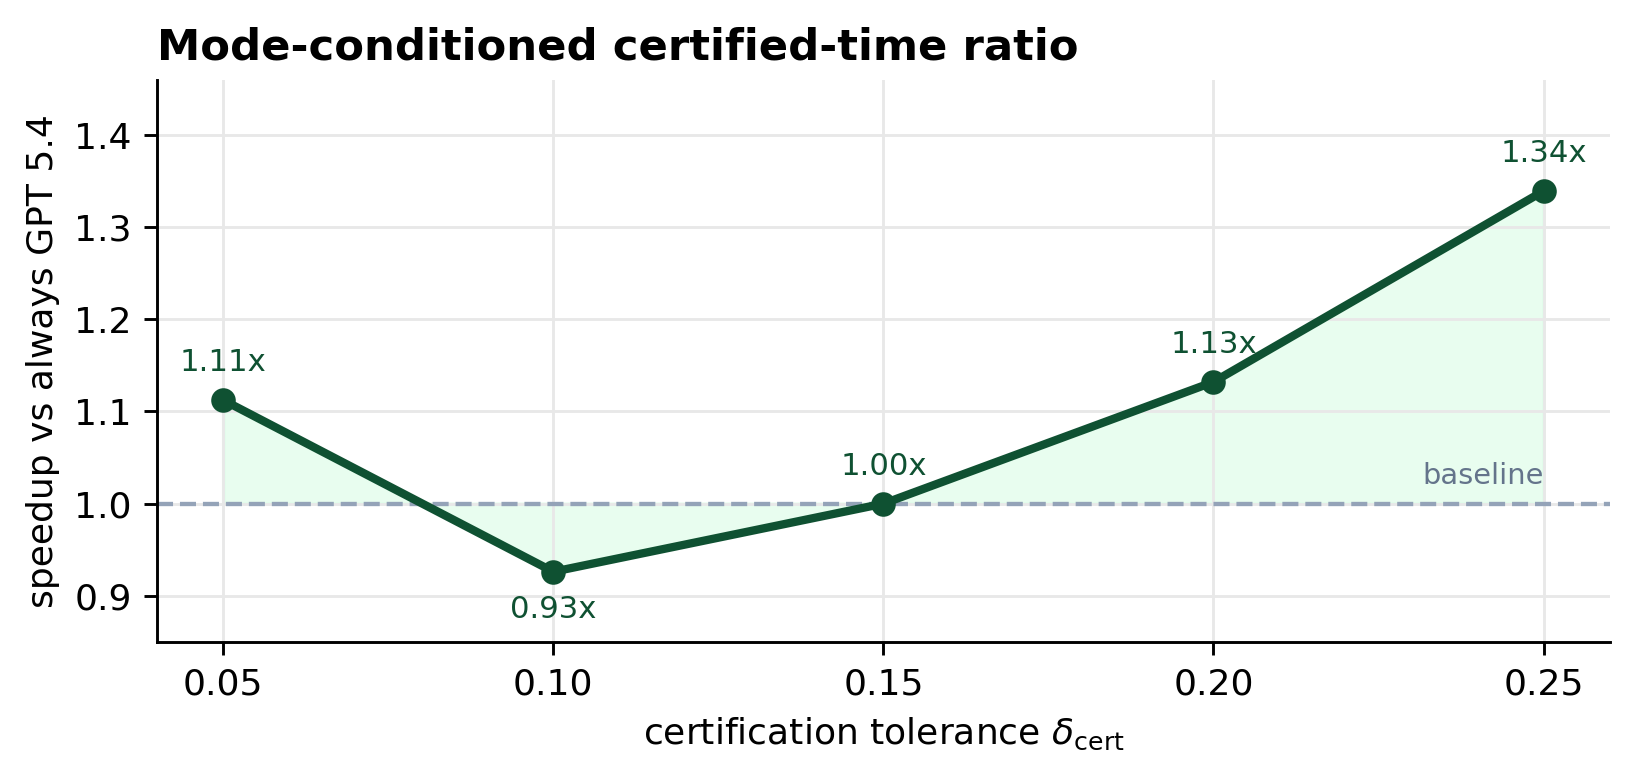
\includegraphics[width=\linewidth]{figures/autoresearch/certified_resource_summary_unified.png}
\caption{Certified-time ratio for the mode-conditioned policy induced by Table~\ref{tab:worker-frontier-accounting}.
The curve compares the factored certified time of the policy \(\{\textit{MLP}\mapsto\textit{GPT 5.4},\textit{CNN}\mapsto\textit{GPT 5.4 Mini},\textit{ResNet}\mapsto\textit{GPT 5.3 Codex}\}\) against the best pooled always-agent baseline, \textit{GPT 5.4}.
Values above one indicate lower certified time for the mode-conditioned policy.}
\label{fig:certified-resource-summary}
\end{figure}

\paragraph{Experiment 2: Candidate-agent scout signals.}
We next ask whether start-of-run information can move a router toward the right agent system.
This audit uses the balanced \(n=30\) panel restricted to shared seeds across modes, giving 30 task instances.
For each instance, the router chooses among \(\{\textit{GPT 5.3 Codex},\textit{GPT 5.4},\textit{GPT 5.4 Mini}\}\).
We evaluate three router models, \(\texttt{gpt\_5\_5\_router\_xhigh}\), \(\texttt{gpt\_5\_4\_router\_xhigh}\), and \(\texttt{gpt\_5\_4\_mini\_router\_xhigh}\), under three incrementally informative start-of-run records:
\(Z_0\) contains only the deployment contract and candidate agent systems;
\(Z_1\) adds the initial \texttt{train.py} and static workload description;
and \(Z_2\) adds two edit--verify scout steps for every candidate agent system.
\sout{The scout prefix is evidence for selection only: the selected agent system is still evaluated by its full trajectory, and the router never observes full-horizon outcomes.}

The full-horizon outcome table already shows why this is a nontrivial routing problem.
On these 30 instances, the always-\texttt{gpt\_5\_4} policy succeeds on \(30/30\) runs and has mean best-visible validation loss \(1.192\).
\texttt{gpt\_5\_3\_codex} succeeds on \(29/30\), with mean loss \(1.396\), while \texttt{gpt\_5\_4\_mini} succeeds on \(28/30\), with mean loss \(1.262\).
The per-instance full-horizon oracle has mean loss \(1.113\), choosing \texttt{gpt\_5\_4} on 18 instances and \texttt{gpt\_5\_4\_mini} on 12; it never chooses \texttt{gpt\_5\_3\_codex}.
Thus the best always-worker baseline is strong, but there is still instance-level headroom.
The oracle here is retrospective: for each shared instance \(x\), it is the worker with the lowest full-horizon best-visible validation loss among the three complete worker trajectories.
It is not visible to the router and is used only to test whether progressively richer pre-deployment evidence points the router toward the worker that actually performs best on that instance.

We also run an allocation-output version of the router audit for the two completed frontier routers, asking each router to report a mode posterior \(\pi_z\), a mode-allocation vector \(q_z\), and a hard selected agent system.
Figure~\ref{fig:router-shift-lookup-summary} summarizes the resulting diagnostic.
The left panel shows that \(Z_0\) correctly behaves like an uninformative balanced record, while \(Z_1\) and \(Z_2\) move both posterior mass and allocation mass toward the predeclared architecture mode.
The right panel overlays two decision rules: open markers are the router's direct hard worker choices, and filled markers are the choices induced by applying the frozen mode--system certified-resource table from Experiment 1 to the router posterior.
This comparison shows that mode recognition does not by itself make the direct worker choice stable; the lookup-calibrated decision exposes the intended separation between recognizing the mode and choosing the agent system.

\begin{figure}[t]
\centering
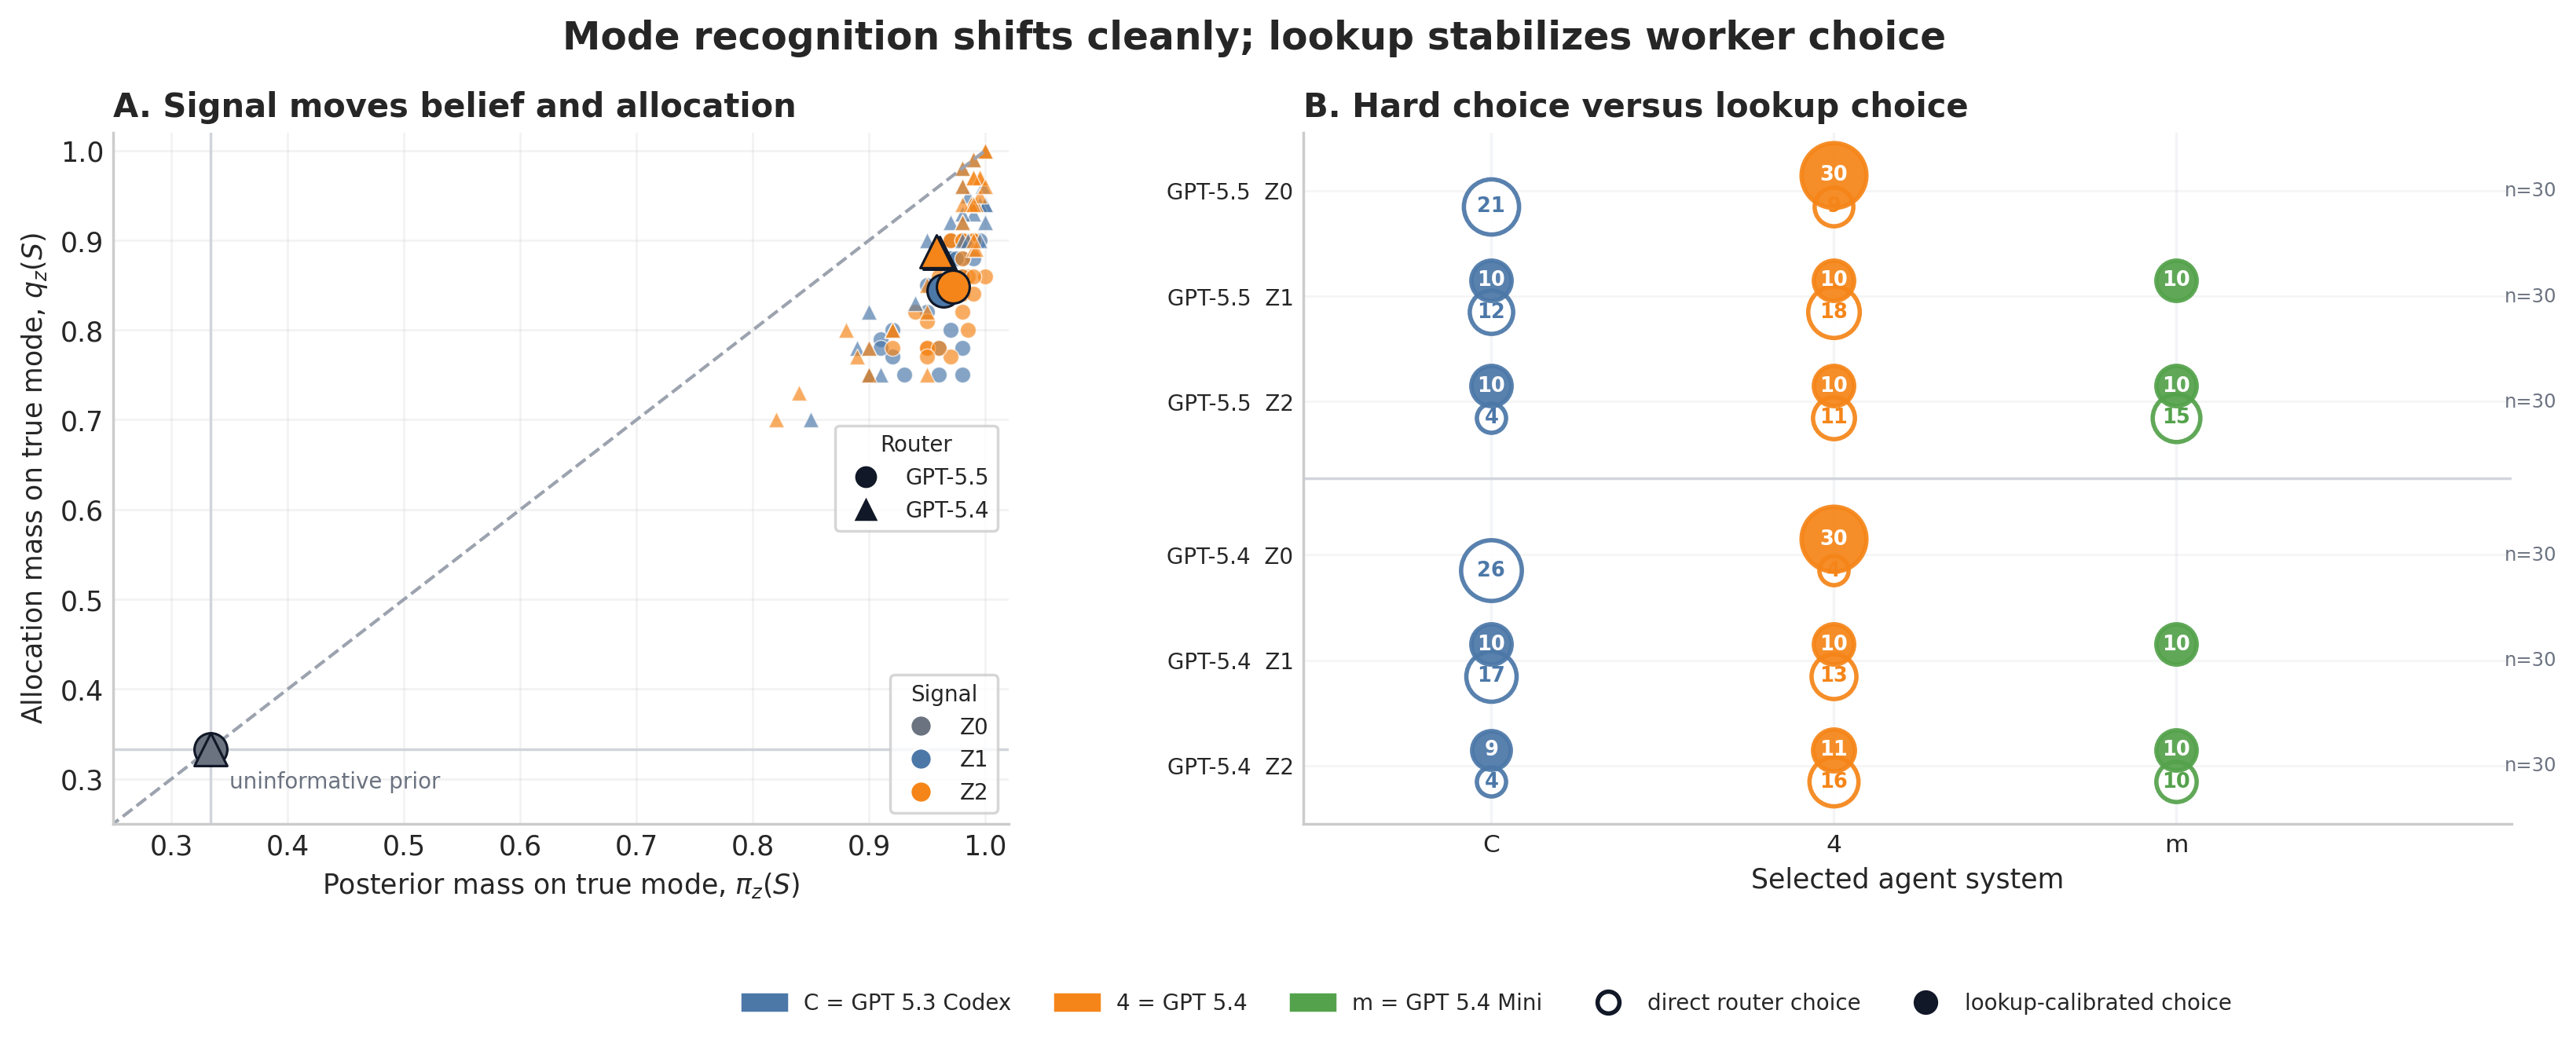
\includegraphics[width=\linewidth]{figures/autoresearch/router_shift_lookup_summary.png}
\caption{Single-figure audit of mode recognition and worker choice for the allocation-output router protocol.
Panel A plots, for each instance, posterior mass on the true architecture mode against allocation mass on the same mode; large markers are signal-level means.
Panel B compares direct hard worker choices with lookup-calibrated choices: rows are router--signal pairs, columns are agent systems, open markers denote direct router choices, filled markers denote lookup-calibrated choices, and marker area scales with the number of selected instances.
Counts are shown for the completed \(\texttt{gpt\_5\_5\_router\_xhigh}\) and \(\texttt{gpt\_5\_4\_router\_xhigh}\) allocation-output audits.}
\label{fig:router-shift-lookup-summary}
\end{figure}

\begin{table}[t]
\centering
\small
\setlength{\tabcolsep}{3.5pt}
\caption{Candidate-agent scout routing audit on the balanced \(n=30\) panel.
Selection counts are ordered \(C/4/m\), where \(C=\texttt{gpt\_5\_3\_codex}\), \(4=\texttt{gpt\_5\_4}\), and \(m=\texttt{gpt\_5\_4\_mini}\).
Oracle hit means the selected agent system matches the per-instance agent system with the lowest full-horizon best-visible validation loss.
Regret is the selected loss minus that oracle loss.}
\label{tab:candidate-scout-router}
\resizebox{\linewidth}{!}{%
\begin{tabular}{@{}llrrrrrr@{}}
\toprule
Router & Signal & Select \(C/4/m\) & Oracle hit & Success & Mean loss & Regret & Mean cost \\
\midrule
\texttt{gpt\_5\_4\_router\_xhigh} & \(Z_0\) & \(26/4/0\) & 3/30 & 30/30 & 1.377 & 0.264 & 483 \\
\texttt{gpt\_5\_4\_router\_xhigh} & \(Z_1\) & \(19/11/0\) & 7/30 & 29/30 & 1.298 & 0.185 & 973 \\
\texttt{gpt\_5\_4\_router\_xhigh} & \(Z_2\) & \(3/13/14\) & \textbf{21/30} & 30/30 & \textbf{1.160} & \textbf{0.047} & 2228 \\
\texttt{gpt\_5\_5\_router\_xhigh} & \(Z_0\) & \(30/0/0\) & 0/30 & 29/30 & 1.396 & 0.283 & 429 \\
\texttt{gpt\_5\_5\_router\_xhigh} & \(Z_1\) & \(28/2/0\) & 0/30 & 29/30 & 1.394 & 0.280 & 446 \\
\texttt{gpt\_5\_5\_router\_xhigh} & \(Z_2\) & \(4/11/15\) & 19/30 & 29/30 & 1.180 & 0.066 & 2204 \\
\texttt{gpt\_5\_4\_mini\_router\_xhigh} & \(Z_0\) & \(6/24/0\) & 16/30 & 30/30 & 1.236 & 0.123 & 1263 \\
\texttt{gpt\_5\_4\_mini\_router\_xhigh} & \(Z_1\) & \(2/27/1\) & 16/30 & 30/30 & 1.205 & 0.092 & 1556 \\
\texttt{gpt\_5\_4\_mini\_router\_xhigh} & \(Z_2\) & \(4/18/8\) & 19/30 & 30/30 & 1.189 & 0.076 & 1656 \\
\bottomrule
\end{tabular}}
\end{table}

\begin{table}[t]
\centering
\small
\setlength{\tabcolsep}{3.5pt}
\caption{Oracle-alignment gain from progressively richer router records.
Oracle hit means that the selected worker matches the per-instance full-horizon quality oracle from Table~\ref{tab:candidate-scout-router}.
Shift is measured relative to each router's \(Z_0\) decision on the same instance.
The aggregate rows pool the three routers, for \(90\) decisions per signal level.}
\label{tab:oracle-alignment-by-signal}
\resizebox{\linewidth}{!}{%
\begin{tabular}{@{}lcccccc@{}}
\toprule
Router & Signal & Oracle hit & Hit rate & Mean regret & Shift vs.\ \(Z_0\) & Selected \(C/4/m\) \\
\midrule
\texttt{gpt\_5\_4\_mini\_router\_xhigh} & \(Z_0\) & 16/30 & 0.533 & 0.123 & -- & \(6/24/0\) \\
\texttt{gpt\_5\_4\_mini\_router\_xhigh} & \(Z_1\) & 16/30 & 0.533 & 0.092 & 8/30 & \(2/27/1\) \\
\texttt{gpt\_5\_4\_mini\_router\_xhigh} & \(Z_2\) & 19/30 & 0.633 & 0.076 & 13/30 & \(4/18/8\) \\
\midrule
\texttt{gpt\_5\_4\_router\_xhigh} & \(Z_0\) & 3/30 & 0.100 & 0.264 & -- & \(26/4/0\) \\
\texttt{gpt\_5\_4\_router\_xhigh} & \(Z_1\) & 7/30 & 0.233 & 0.185 & 15/30 & \(19/11/0\) \\
\texttt{gpt\_5\_4\_router\_xhigh} & \(Z_2\) & \textbf{21/30} & \textbf{0.700} & \textbf{0.047} & 24/30 & \(3/13/14\) \\
\midrule
\texttt{gpt\_5\_5\_router\_xhigh} & \(Z_0\) & 0/30 & 0.000 & 0.283 & -- & \(30/0/0\) \\
\texttt{gpt\_5\_5\_router\_xhigh} & \(Z_1\) & 0/30 & 0.000 & 0.280 & 2/30 & \(28/2/0\) \\
\texttt{gpt\_5\_5\_router\_xhigh} & \(Z_2\) & 19/30 & 0.633 & 0.066 & 26/30 & \(4/11/15\) \\
\midrule
All routers & \(Z_0\) & 19/90 & 0.211 & 0.223 & -- & \(62/28/0\) \\
All routers & \(Z_1\) & 23/90 & 0.256 & 0.186 & 25/90 & \(49/40/1\) \\
All routers & \(Z_2\) & \textbf{59/90} & \textbf{0.656} & \textbf{0.063} & 63/90 & \(11/42/37\) \\
\bottomrule
\end{tabular}}
\end{table}

\paragraph{Experiment 3: Routing response and quality gain.}
Tables~\ref{tab:candidate-scout-router} and~\ref{tab:oracle-alignment-by-signal} show that the scout record changes the qualitative behavior of the routers and improves their alignment with the per-instance full-horizon oracle.
Without scout evidence, \texttt{gpt\_5\_5\_router\_xhigh} and \texttt{gpt\_5\_4\_router\_xhigh} are overly conservative and route mostly to \texttt{gpt\_5\_3\_codex}, despite \texttt{gpt\_5\_3\_codex} never being the full-horizon oracle on this panel.
Adding static code in \(Z_1\) helps only modestly.
Adding candidate-agent scout traces in \(Z_2\) moves all three routers toward the two workers that actually occupy the full-horizon oracle frontier.
The best setting is \(\texttt{gpt\_5\_4\_router\_xhigh}\) with \(Z_2\): it selects \(C/4/m=3/13/14\), matches the oracle worker on \(21/30\) instances, succeeds on \(30/30\), and reduces mean full-horizon loss to \(1.160\).
This beats the best always-worker baseline, \texttt{gpt\_5\_4}, by \(0.032\) mean loss and closes much of the gap to the per-instance oracle at \(1.113\).
Pooling across the three router models, oracle hits increase from \(19/90\) under \(Z_0\) to \(23/90\) under \(Z_1\) and \(59/90\) under \(Z_2\), while mean full-horizon regret drops from \(0.223\) to \(0.186\) and then to \(0.063\).
Thus the improvement is not merely that routers change their output more often: the changes induced by candidate-agent scouts are directionally aligned with the worker that later achieves the best full-horizon validation loss on the same instance.

The improvement is specifically tied to candidate-level evidence.
Across the three routers, \(Z_2\) decisions are unanimous on \(22/30\) instances and split two-to-one on the remaining eight; no instance produces three different selected workers.
In contrast, \(Z_0\) and \(Z_1\) are dominated by router priors and disagree mainly over how much to prefer the cheaper coding-specialized worker.
This is the mechanism predicted by the framework: richer information is useful when it changes allocation toward actions with better realized instance-level cost--quality profiles.

\paragraph{Experiment 4: Deployment interpretation.}
\sout{The candidate-scout result is positive but not yet a free-standing deployment recommendation.}
First, Table~\ref{tab:candidate-scout-router} is a full-horizon best-loss audit on an existing balanced trajectory panel, not a fresh paired deployment experiment with independent selected-worker reruns.
Second, the reported mean cost is the selected worker's full-run accounting cost; it does not yet include the measurement cost of running all candidate scouts before selection.

Third, the best routing setting improves quality relative to the best always-worker baseline while increasing selected-run cost.
Therefore the result validates the information and allocation mechanism, but the final deployment claim still requires the paired net-gain estimand in~\eqref{eq:router-gain} with scout costs charged explicitly.
The main conclusion is correspondingly conditional: candidate-agent scout traces can make prompt-only routing useful on this panel, while deployment promotion depends on whether their measurement cost is worth paying.



\section{Related work}
\label{sec:related}

The closest classical ancestor is algorithm selection.
Since Rice's formulation, solver portfolios have treated performance as instance-dependent: SATzilla and AutoFolio learn to select solvers from instance features rather than report one globally best solver~\citep{rice1976algorithm,xu2012satzilla,lindauer2015autofolio,kotthoff2016algorithm}.
Our contribution is the specialization to externally verified LLM agents, where a router observes a controlled pre-deployment record and is scored by paired deployment loss rather than standalone routing accuracy.
Unlike AutoML systems such as auto-sklearn, which tune pipelines offline for a dataset, our unit is a deployable action for a concrete verifier-backed instance~\citep{feurer2015autosklearn}.

LLM routing and cascades provide the model-menu context.
FrugalGPT, RouteLLM, RouterBench, LLMRouterBench, and compound-system routers study cost-quality routing over heterogeneous model pools~\citep{chen2023frugalgpt,ong2024routellm,hu2024routerbench,anonymous2026llmrouterbench,chen2025optimizing,yue2025masrouter,zaharia2024compound}.
We ask how much verified, task-specific information is worth before committing to an expensive agentic deployment.

Verified agent benchmarks provide the task substrate.
SWE-bench evaluates repository repair against tests, AutoResearch evaluates training-loop edits against validation feedback, and theorem-proving systems use analogous external validators~\citep{jimenez2024swebench,karpathy2026autoresearch}.
Repeated sampling and inference-time scaling further show that lower-cost or smaller models can become competitive when verification is available~\citep{brown2024monkeys,snell2025testtime,wu2025inference,osca2024}.
Our question is upstream of the launched worker: which action should be selected, what should the router observe, and how should that observation be charged?

\section{Discussion and limitations}
\label{sec:discussion}

The paper separates a theory-facing diagnostic claim from a deployment-facing validation claim.
The experiments support the diagnostic claim: first-passage speed, final improvement, certified log-effort, full-horizon quality, and deployment loss disagree on the same verified task family.
They also show that the form of pre-deployment information matters.
Static task descriptions alone mostly preserve router priors, while candidate-agent scout traces provide actionable instance-level evidence.
Across the three prompt-only routers, the contract-only record \(Z_0\) matches the per-instance full-horizon oracle on only \(19/90\) decisions; adding the static program in \(Z_1\) gives \(23/90\); adding two-step candidate scouts in \(Z_2\) gives \(59/90\).
The same progression reduces mean full-horizon oracle regret from \(0.223\) to \(0.186\) and then to \(0.063\).
In the strongest audit, \(\texttt{gpt\_5\_4\_router\_xhigh}\) with \(Z_2\) matches the oracle worker on \(21/30\) instances, beats the best always-worker baseline in mean best-visible validation loss, and substantially reduces oracle regret.
This is evidence for the information-allocation mechanism: interacting briefly with the task through candidate-agent scouts helps routers choose the worker that will perform best on that instance.
It is not yet an unqualified deployment policy because the audit reuses an existing balanced trajectory table, and the scout measurement cost must still be charged in a fresh paired net-gain evaluation.

The main limitations are the packed-mode abstraction, the fixed executable prototypes, and the small three-worker action menu.
Real agent trajectories are stateful, task modes may be fuzzy, and the reported quantities are fixed-panel diagnostics rather than population-level deployment estimates.
This is why the appendix reports threshold curves, occupancy, cost sensitivity, token accounting, router-record checks, and signal-ablation diagnostics instead of treating the finite-mode surrogate as sufficient.
The decomposition is therefore a claim discipline: it helps identify cost, competence, information, and allocation mechanisms, but paired deployment gain decides whether a routing recommendation is deployable.

\paragraph{Future work.}
The immediate experimental extension is to rerun the candidate-scout router as a fresh paired deployment study: run the scouts, sample independent selected-worker trajectories from scratch, and subtract scout wall-clock, token, and context costs.
A second extension is to train or constrain routers against the deployment-loss frontier rather than only prompt them with records.
The current \texttt{gpt\_5\_4\_mini} panel already shows a retry-crossover regime on \textit{compact CNN}, but richer menus are needed to test whether lower-cost workers can reliably compensate for lower one-attempt success across more task families.
Beyond this benchmark, repository repair, theorem checking, and multi-file research-code editing would test less artificial mode schemas and more heterogeneous measurement costs.

\paragraph{Conclusion.}
Model choice inside an agent harness is not a scalar leaderboard problem.
It is a budget-aware deployment decision validated by paired outcomes after measurement cost.
The three-worker study makes this concrete.
The worker frontier rejects a single global ranking, and the candidate-scout audit shows that richer pre-deployment evidence can change routing in the right direction: with \(Z_2\), routers collectively move from \(19/90\) to \(59/90\) per-instance oracle hits, and the best \(Z_2\) router beats the best always-worker baseline in full-horizon quality on the balanced panel.
The remaining gate is deployment accounting.
A measurement or router should be promoted only when it changes selected actions in a way that improves paired verified deployment loss under the declared resource convention, with the cost of buying the information included.

\clearpage
\bibliographystyle{unsrtnat}
\bibliography{references}

\clearpage

\appendix


% ============================================================
% APPENDIX PATCH
% ============================================================

\clearpage
\section{Proofs: certified-time derivation of log-effort}
\label{app:proofs}
\label{app:certified-log-effort}
\label{app:proofs}

This appendix derives the log-effort identity used in Section~\ref{sec:accounting}.
The main text uses three objects:
\[
    \overline T_M(\delta_{\mathrm{cert}})
    \quad\text{global certified time,}
    \qquad
    \mathsf T_{M,q}(s,z)
    \quad\text{packed mode-conditioned time,}
\]
and the packed identity of Theorem~\ref{thm:four-term}.
The notation \(\overline T\) is reserved for certified-time quantiles; the symbol
\(\mathsf T\) denotes the packed time-sharing model whose expected logarithm decomposes
algebraically.

\subsection{Coding-gain bound}

Let \(\mathfrak A\) be a countable prefix-coded class of admissible solvers.  For
\(B\in\mathfrak A\), let \(t_B(\delta_{\mathrm{cert}})\) denote its certified time at
confidence level \(\delta_{\mathrm{cert}}\).  A baseline universal scheduler assigns Kraft
weights \(w(B)\), while a conditioned scheduler, after observing a signal value \(Z=z\),
assigns Kraft weights \(w(B\mid z)\).  Thus
\[
    \sum_{B\in\mathfrak A}w(B)\le 1,
    \qquad
    \sum_{B\in\mathfrak A}w(B\mid z)\le 1.
\]
Giving solver \(B\) only share \(w(B)\) of the wall-clock means that \(B\) receives
\(t_B\) units of internal computation after \(t_B/w(B)\) wall-clock units.  Hence
\[
    \overline T_U
    =
    c_{\mathrm{sim}}
    \inf_{B\in\mathfrak A}
    \frac{t_B(\delta_{\mathrm{cert}})}{w(B)},
    \qquad
    \overline T_{U\mid z}
    =
    c_{\mathrm{sim}}
    \inf_{B\in\mathfrak A}
    \frac{t_B(\delta_{\mathrm{cert}})}{w(B\mid z)}.
\]

\begin{proposition}[Coding-gain bound]
\label{prop:app-coding-gain}
Fix a realized signal value \(z\), and let
\[
    B_z^\star
    \in
    \argmin_{B\in\mathfrak A}
    \frac{t_B(\delta_{\mathrm{cert}})}{w(B\mid z)}.
\]
Then
\[
    \log\frac{\overline T_U}{\overline T_{U\mid z}}
    \le
    \log\frac{w(B_z^\star\mid z)}{w(B_z^\star)}.
\]
\end{proposition}

\begin{proof}
By definition of \(B_z^\star\),
\[
    \overline T_{U\mid z}
    =
    c_{\mathrm{sim}}
    \frac{t_{B_z^\star}(\delta_{\mathrm{cert}})}
         {w(B_z^\star\mid z)}.
\]
Since \(\overline T_U\) is an infimum over the same admissible solver class,
\[
    \overline T_U
    \le
    c_{\mathrm{sim}}
    \frac{t_{B_z^\star}(\delta_{\mathrm{cert}})}
         {w(B_z^\star)}.
\]
Dividing cancels \(c_{\mathrm{sim}}\) and \(t_{B_z^\star}(\delta_{\mathrm{cert}})\), giving
\[
    \frac{\overline T_U}{\overline T_{U\mid z}}
    \le
    \frac{w(B_z^\star\mid z)}{w(B_z^\star)}.
\]
Taking logarithms proves the claim.
\end{proof}

This is the basic coding interpretation of certified speedup: side information helps only
by moving scheduler weight toward solvers that are useful for the realized instance.

\subsection{Optional resource-bounded information form}

The previous bound is pointwise and does not require a structure variable.
To express it as a resource-bounded information bound, one needs an aligned witness class.

\begin{definition}[Resource-bounded structure length]
\label{def:app-ipoly}
Let \(H_{\mathrm{str}}\) denote reusable task structure, and let
\[
    \mathfrak A(H_{\mathrm{str}})\subseteq \mathfrak A
\]
be a nonempty class of solvers realizing that structure.  Define
\[
    K^{\mathrm{poly}}(H_{\mathrm{str}})
    :=
    \inf_{B\in\mathfrak A(H_{\mathrm{str}})}
    \{-\log w(B)\},
\]
\[
    K^{\mathrm{poly}}(H_{\mathrm{str}}\mid z)
    :=
    \inf_{B\in\mathfrak A(H_{\mathrm{str}})}
    \{-\log w(B\mid z)\},
\]
and
\[
    I_{\mathrm{poly}}(H_{\mathrm{str}}:z)
    :=
    K^{\mathrm{poly}}(H_{\mathrm{str}})
    -
    K^{\mathrm{poly}}(H_{\mathrm{str}}\mid z).
\]
\end{definition}

\begin{assumption}[Aligned witness]
\label{ass:app-aligned-witness}
For each realized \(z\), there exists
\(B_H(z)\in\mathfrak A(H_{\mathrm{str}})\) such that
\[
    \log\frac{t_{B_H}(\delta_{\mathrm{cert}})}{w(B_H\mid z)}
    \le
    \inf_{B\in\mathfrak A}
    \log\frac{t_B(\delta_{\mathrm{cert}})}{w(B\mid z)}
    +
    \rho_z,
\]
and
\[
    -\log w(B_H)
    \le
    K^{\mathrm{poly}}(H_{\mathrm{str}})+\chi_z.
\]
The first inequality says that the structure witness is nearly conditionally optimal.
The second says that the same witness is not much longer than the shortest prior-coded
solver realizing the structure.
\end{assumption}

\begin{proposition}[Resource-bounded information upper bound]
\label{prop:app-ipoly-bound}
Under Assumption~\ref{ass:app-aligned-witness},
\[
    \log\frac{\overline T_U}{\overline T_{U\mid z}}
    \le
    I_{\mathrm{poly}}(H_{\mathrm{str}}:z)+\chi_z+\rho_z.
\]
\end{proposition}

\begin{proof}
Let
\[
    L_U:=\inf_{B\in\mathfrak A}\{\log t_B-\log w(B)\},
    \qquad
    L_z:=\inf_{B\in\mathfrak A}\{\log t_B-\log w(B\mid z)\}.
\]
The simulation overhead cancels, so
\[
    \log\frac{\overline T_U}{\overline T_{U\mid z}}
    =
    L_U-L_z.
\]
For \(B_H=B_H(z)\),
\[
    L_U
    \le
    \log t_{B_H}-\log w(B_H),
\]
and Assumption~\ref{ass:app-aligned-witness} gives
\[
    L_z
    \ge
    \log t_{B_H}-\log w(B_H\mid z)-\rho_z.
\]
Therefore
\[
\begin{aligned}
    L_U-L_z
    &\le
    -\log w(B_H)+\log w(B_H\mid z)+\rho_z.
\end{aligned}
\]
Using
\[
    -\log w(B_H)
    \le
    K^{\mathrm{poly}}(H_{\mathrm{str}})+\chi_z
\]
and
\[
    \log w(B_H\mid z)
    \le
    -K^{\mathrm{poly}}(H_{\mathrm{str}}\mid z),
\]
we get
\[
    L_U-L_z
    \le
    K^{\mathrm{poly}}(H_{\mathrm{str}})
    -
    K^{\mathrm{poly}}(H_{\mathrm{str}}\mid z)
    +
    \chi_z+\rho_z.
\]
This is the claimed bound.
\end{proof}

\begin{remark}[Why this assumption is explicit]
The coding-gain bound in Proposition~\ref{prop:app-coding-gain} holds without a structure
variable.  The \(I_{\mathrm{poly}}\) form does not.  It requires the solver accelerated by
\(z\) to be represented by a near-optimal witness in the chosen reusable-structure class.
Without this alignment, side information may favor a solver unrelated to
\(H_{\mathrm{str}}\), and the information upper bound need not follow.
\end{remark}

\subsection{Proper time and inverse-share expansion}
\label{app:proper-time-inverse-share}

The packed-time law is the time-sharing expansion of focused certified time.
For mode \(s\), \(t_0(M,s)\) is the focused certified scale of system \(M\): the time
scale needed when all mode-relevant effort is assigned to the correct strategy.
If the packed scheduler assigns that strategy only clock-rate share \(q_z(s)\), then the
same focused computation is accumulated after time
\[
    \frac{t_0(M,s)}{q_z(s)}.
\]
Including scalar unit cost and shared simulation overhead gives
\[
    \mathsf T_{M,q}(s,z)
    =
    c_{\mathrm{sim}}\,
    \kappa(M,s)\,
    \frac{t_0(M,s)}{q_z(s)}.
\]
Thus the inverse-share factor is not a separate success-probability heuristic.
The modeling assumption is the finite packed representation: that the workload is
adequately described by a finite dictionary of solver-relevant modes and mode-specialized
strategies.

\subsection{Conditional packed log-time}

\begin{lemma}[Conditional packed log-time]
\label{lem:app-conditional-packed}
Under Assumption~\ref{ass:packed}, for every realized signal \(Z=z\),
\[
\begin{aligned}
    \E_{S\sim\pi_z}
    \bigl[
        \log \mathsf T_{M,q}(S,z)
    \bigr]
    &=
    \log c_{\mathrm{sim}}
    +
    \E_{S\sim\pi_z}[\log\kappa(M,S)]
    +
    \E_{S\sim\pi_z}[\log t_0(M,S)]
    \\
    &\quad
    +
    H(\pi_z)
    +
    \KL(\pi_z\|q_z).
\end{aligned}
\]
For fixed \(M\) and \(z\), the minimizing share vector is
\[
    q_z^\star=\pi_z,
\]
on the support of \(\pi_z\), and the excess conditional expected log-time of any other
\(q_z\) is exactly
\[
    \KL(\pi_z\|q_z).
\]
\end{lemma}

\begin{proof}
By Assumption~\ref{ass:packed},
\[
    \log \mathsf T_{M,q}(s,z)
    =
    \log c_{\mathrm{sim}}
    +
    \log\kappa(M,s)
    +
    \log t_0(M,s)
    -
    \log q_z(s).
\]
Taking expectation over \(S\sim\pi_z\), the only nontrivial term is
\[
    \E_{S\sim\pi_z}[-\log q_z(S)]
    =
    \sum_s \pi_z(s)\log\frac{1}{q_z(s)}.
\]
The cross-entropy identity gives
\[
    \sum_s \pi_z(s)\log\frac{1}{q_z(s)}
    =
    H(\pi_z)+\KL(\pi_z\|q_z).
\]
Nonnegativity of KL gives optimality, with equality exactly when \(q_z=\pi_z\) on the
support of \(\pi_z\).
\end{proof}

\subsection{Proof of the packed-mode certified log-speedup identity}

\begin{proof}[Proof of Theorem~\ref{thm:four-term}]
For the baseline system \((M_0,q_0)\), Lemma~\ref{lem:app-conditional-packed} with no
signal conditioning gives
\[
\begin{aligned}
    \E[\log \mathsf T_{M_0,q_0}(S)]
    &=
    \log c_{\mathrm{sim}}
    +
    \E_{S\sim\pi}[\log\kappa(M_0,S)]
    +
    \E_{S\sim\pi}[\log t_0(M_0,S)]
    \\
    &\quad
    +
    H(\pi)
    +
    \KL(\pi\|q_0).
\end{aligned}
\]
For the routed packed system \((M,q)\),
\[
\begin{aligned}
    \E[\log \mathsf T_{M,q}(S,Z)]
    &=
    \log c_{\mathrm{sim}}
    +
    \E_{S\sim\pi}[\log\kappa(M,S)]
    +
    \E_{S\sim\pi}[\log t_0(M,S)]
    \\
    &\quad
    +
    \E_ZH(\pi_Z)
    +
    \E_Z\KL(\pi_Z\|q_Z).
\end{aligned}
\]
Here we used the tower property for the mode-conditioned terms:
\[
    \E_Z\E_{S\sim\pi_Z}[\log\kappa(M,S)]
    =
    \E_{S\sim\pi}[\log\kappa(M,S)],
    \qquad
    \E_Z\E_{S\sim\pi_Z}[\log t_0(M,S)]
    =
    \E_{S\sim\pi}[\log t_0(M,S)].
\]
Subtracting the routed expression from the baseline expression cancels the shared
\(\log c_{\mathrm{sim}}\) and yields
\[
\begin{aligned}
&\E[
    \log \mathsf T_{M_0,q_0}(S)
    -
    \log \mathsf T_{M,q}(S,Z)
]
\\
&\quad =
\E_{S\sim\pi}
\left[
    \log\frac{\kappa(M_0,S)}{\kappa(M,S)}
\right]
+
\E_{S\sim\pi}
\left[
    \log\frac{t_0(M_0,S)}{t_0(M,S)}
\right]
+
H(\pi)-\E_ZH(\pi_Z)
+
\KL(\pi\|q_0)
-
\E_Z\KL(\pi_Z\|q_Z).
\end{aligned}
\]
Since
\[
    H(\pi)-\E_ZH(\pi_Z)=\MI_\pi(S;Z),
\]
we obtain
\[
\begin{aligned}
&\E[
    \log \mathsf T_{M_0,q_0}(S)
    -
    \log \mathsf T_{M,q}(S,Z)
]
\\
&\quad =
\E_{S\sim\pi}
\left[
    \log\frac{\kappa(M_0,S)}{\kappa(M,S)}
\right]
+
\E_{S\sim\pi}
\left[
    \log\frac{t_0(M_0,S)}{t_0(M,S)}
\right]
+
\MI_\pi(S;Z)
+
\KL(\pi\|q_0)
-
\E_Z\KL(\pi_Z\|q_Z).
\end{aligned}
\]
This proves the general identity.  The prior-matched case \(q_0=\pi\) follows because
\[
    \KL(\pi\|\pi)=0.
\]
\end{proof}

\subsection{Success-hazard specialization}

The identity above is exact in terms of the focused certified scale \(t_0(M,s)\).
The familiar success-probability form is a specialization.

Suppose independent attempts of system \(M\) on mode \(s\) succeed with probability
\(p_M(s)\in(0,1)\), and suppose one attempt has normalized unit duration \(u_M(s)\).
After \(N\) attempts, the success probability is
\[
    1-(1-p_M(s))^N.
\]
To achieve failure probability at most \(\delta_{\mathrm{cert}}\), it suffices and is necessary that
\[
    N
    \ge
    \frac{\log(1/\delta_{\mathrm{cert}})}
         {-\log(1-p_M(s))}.
\]
Thus the exact geometric certified scale is
\[
    t_0(M,s,\delta_{\mathrm{cert}})
    =
    u_M(s)
    \left\lceil
    \frac{\log(1/\delta_{\mathrm{cert}})}
         {-\log(1-p_M(s))}
    \right\rceil.
\]
Let
\[
    h_M(s):=-\log(1-p_M(s))
\]
be the verified success hazard.  Then, up to unit-duration and confidence constants,
\[
    t_0(M,s)\propto \frac{1}{h_M(s)}.
\]
When \(p_M(s)\) is small, or when \(p_M(s)\) is used as an effective verified success
hazard,
\[
    h_M(s)\approx p_M(s),
    \qquad
    t_0(M,s)\propto\frac{1}{p_M(s)}.
\]
In that specialization,
\[
    \log\frac{t_0(M_0,s)}{t_0(M,s)}
    =
    \log\frac{p_M(s)}{p_{M_0}(s)}
\]
up to constants independent of the comparison.

\begin{remark}[Hazard versus raw success probability]
When \(p_M(s)\) is not small, the exact scale is governed by
\[
    -\log(1-p_M(s)),
\]
not by \(p_M(s)\) itself.  The main-text notation \(p_M(s)\) should therefore be read
as an effective verified success hazard or as the small-\(p\) geometric-trials approximation.
\end{remark}

\subsection{Retry crossover design rule}
\label{app:retry-crossover}

\begin{theorem}[Single-mode retry crossover]
\label{thm:crossover}
Fix a single homogeneous mode, success threshold \(\gamma\), and horizon \(H\).
Let a stronger system \(M_h\) have one-attempt first-passage success probability
\[
    p_h=\Pr[\tau_\gamma(M_h,X)\le H]
\]
and expected first-passage cost \(\kappa_h\).  Let a cheaper system \(M_\ell\) have
\[
    p_\ell=\Pr[\tau_\gamma(M_\ell,X)\le H],
    \qquad
    0<p_\ell<p_h<1,
\]
and expected first-passage cost \(\kappa_\ell<\kappa_h\).
Assume retries of \(M_\ell\) are conditionally independent fresh attempts with the same
one-attempt horizon \(H\) and success probability \(p_\ell\).  The retry depth that matches
the stronger system's one-attempt success probability is
\[
    D_{\mathrm{cross}}
    =
    \frac{\log(1-p_h)}{\log(1-p_\ell)}.
\]
The corresponding fixed-depth retry block is cost-favorable whenever
\[
    \left\lceil D_{\mathrm{cross}}\right\rceil\kappa_\ell < \kappa_h .
\]
\end{theorem}

\begin{remark}[Stopping after first retry success]
If retries of \(M_\ell\) stop after the first success and each attempted retry has
unconditional expected cost \(\kappa_\ell\), the expected cost at depth \(D\) is
\[
    \kappa_\ell
    \sum_{d=1}^{D}(1-p_\ell)^{d-1}
    =
    \kappa_\ell\frac{1-(1-p_\ell)^D}{p_\ell}.
\]
The deployment comparison should also account for the residual failure probability under
the chosen loss.  Any within-attempt time-to-success difference is absorbed into
\(\kappa_h\) and \(\kappa_\ell\).
\end{remark}

The multi-mode case is where the packed identity matters.  A cheaper system can be
rational on one mode and irrational on another.  A router is useful only when different
systems win the cost--success tradeoff on different modes and the start-of-run signal helps
identify which mode applies.



\subsection{Finite-horizon empirical surrogate}

In AutoResearch-style experiments, the geometric-trials model is only a motivating limit.
We estimate finite-horizon quantities directly.

For system \(M\), mode \(s\), and horizon \(H\), define
\[
    F_M(s,H):=\Pr(\tau_M\le H\mid S=s),
\]
where \(\tau_M\) is the first verified threshold crossing, and define
\[
    C_M(s,H):=\E[C_{\tau_M\wedge H}\mid M,S=s].
\]
The theorem-facing finite-horizon log-effort loss is
\[
    \ell_{\mathrm{hit}}(M,s;H)
    =
    \log C_M(s,H)-\log(F_M(s,H)\vee\alpha),
\]
where \(\alpha>0\) is a censoring floor.

If first-hit success saturates, we also report a persistence statistic.  For empirical
success threshold \(\gamma\),
\[
    O_M^\gamma(s,H)
    =
    \E\left[
        \frac1H\sum_{h=1}^H
        \one\{G_{M,h}\ge\gamma\}
        \,\middle|\,
        M,S=s
    \right],
\]
and the corresponding operational loss
\[
    \ell_{\mathrm{occ}}(M,s;H)
    =
    \log C_M^H(s,H)-\log(O_M^\gamma(s,H)\vee\alpha).
\]
Here \(C_M^H(s,H)\) is the full no-stop trajectory cost.
This occupancy loss is not the exact packed theorem; it is a deployment diagnostic for
durable verified progress.

\paragraph{Metric guardrail.}
The exact identity decomposes
\[
    \E[\log \mathsf T_{M,q}(S,Z)].
\]
The finite-horizon losses approximate the same cost-divided-by-verified-progress principle,
but they are not equal to the global certified-time quantile
\(\overline T_M(\delta_{\mathrm{cert}})\).
For that reason the experiments report first-hit loss, occupancy loss, survival curves,
hazards, and residual calibration rather than treating a single surrogate as the complete
deployment objective.

\subsection{Approximate packedness and residual term}

The packed identity is exact under the inverse-share time law.  Outside that law, the
right statement is an identity plus a residual.

\begin{assumption}[Approximate packed log-linearity]
\label{ass:app-approx-packed}
Suppose
\[
\begin{aligned}
    \log \mathsf T_{M,q}(s,z)
    &=
    \log c_{\mathrm{sim}}
    +
    \log\kappa(M,s)
    +
    \log t_0(M,s)
    -
    \log q_z(s)
    +
    r_M(s,z,q),
\end{aligned}
\]
with
\[
    |r_M(s,z,q)|\le \eta
\]
uniformly over the evaluated systems, modes, signals, and packed shares.
\end{assumption}

\begin{proposition}[Residual form of the packed identity]
\label{prop:app-residual-decomp}
Under Assumption~\ref{ass:app-approx-packed},
\[
\begin{aligned}
&\E[
    \log \mathsf T_{M_0,q_0}(S)
    -
    \log \mathsf T_{M,q}(S,Z)
]
\\
&\quad =
\E_{S\sim\pi}
\left[
    \log\frac{\kappa(M_0,S)}{\kappa(M,S)}
\right]
+
\E_{S\sim\pi}
\left[
    \log\frac{t_0(M_0,S)}{t_0(M,S)}
\right]
+
\MI_\pi(S;Z)
+
\KL(\pi\|q_0)
-
\E_Z\KL(\pi_Z\|q_Z)
+
R,
\end{aligned}
\]
where
\[
    R=
    \E[r_{M_0}(S,q_0)-r_M(S,Z,q)].
\]
If \(|r_M|\le\eta\) uniformly, then
\[
    |R|\le 2\eta.
\]
\end{proposition}

\begin{proof}
Substitute the approximate log-linear expression into the proof of
Theorem~\ref{thm:four-term}.  The ideal terms decompose exactly as before.  The only
remaining terms are the two residuals:
\[
    R=
    \E[r_{M_0}(S,q_0)-r_M(S,Z,q)].
\]
Uniform boundedness gives
\[
    |R|
    \le
    \E|r_{M_0}(S,q_0)|+\E|r_M(S,Z,q)|
    \le 2\eta.
\]
\end{proof}

The empirical residual
\[
    \widehat{\mathrm{Res}}(d)
    =
    \widehat J_{\mathrm{obs}}(d)-\widehat J_{\mathrm{acct}}(d)
\]
is the practical test of approximate packedness.  Structured residuals by mode, system,
horizon, or router indicate that the finite packed abstraction is missing an interaction.


\section{Operational diagnostics}
\label{subsec:bridge}

The identity above becomes useful only after each term is tied to quantities logged by the deployment protocol.
The verifier-facing progress process is the common object used to operationalize competence, cost, information, and allocation diagnostics.
Fix a horizon $H$ and a task-normalized verified progress process $G_t(a,x)\in[0,1]$ for action $a$ on instance $x$.
In the main experiment, the router acts once before deployment: after observing $Z$, it selects one action, and that action is used for the whole trajectory.
The success and cost diagnostics below are therefore trajectory-level quantities computed from the step-wise verifier trace.
For lower-is-better verifier losses, one admissible normalization is
\[
G_t(a,x)
=
\operatorname{clip}_{[0,1]}\!\left(
\frac{L_0(x)-L_t(a,x)}{|L_0(x)|+\eps_L}
\right),
\]
where $L_0(x)$ is the starting-artifact loss and $L_t(a,x)$ is the verified loss convention at step $t$.
Given a success threshold $\delta>0$,
\[
\tau_\delta(a,x)=\inf\{t\le H:G_t(a,x)\ge \delta\},
\qquad
F_\delta(a,x)=\one\{\tau_\delta(a,x)=\infty\}.
\]
We also log persistence through
\[
\Occ_{\delta,H}(a,x)=\frac{1}{H}\sum_{t=1}^H \one\{G_t(a,x)\ge \delta\}.
\]
The full-horizon audit loss used for persistence and final-quality checks is
\begin{equation}
\ell_{\mathrm{audit}}(a,x;\xi)
=
\ell_{\mathrm{dep}}(a,x;\xi)
+\alpha_{\mathrm{occ}}\bigl(1-\Occ_{\delta,H}(a,x;\xi)\bigr)
+\alpha_{\mathrm{qual}}\psi(G_H(a,x;\xi)),
\label{eq:audit-loss}
\end{equation}
where \(\alpha_{\mathrm{occ}}=\alpha_{\mathrm{qual}}=1\) and \(\psi(u)=1-u\) after clipping \(G_H\in[0,1]\).
It is an audit diagnostic, not the primary deployment loss.

\paragraph{Competence.}
The action competence component $p(a,s)$ is the first-success probability of action $a$ on task mode $s$:
\[
p(a,s)=\Prb[\tau_\delta(a,X)\le H\mid S=s].
\]
Thus $G_t$ is step-wise, but the policy competence term uses the probability that the worker selected by the router reaches the success threshold at least once before the horizon.
Cumulative progress and persistence are not substituted for $p(a,s)$ in the identity.
We log
\[
\bar G_a(s)=\E\!\left[\frac{1}{H}\sum_{t=1}^H G_t(a,X)\mid S=s\right]
\]
and $\Occ_{\delta,H}$ as secondary diagnostics, especially when first-hit success saturates or when partial progress is scientifically relevant.

\paragraph{Cost.}
The action cost component $\kappa(a,s)$ is kept separate from competence.
In the main protocol it is the normalized cost of deploying action $a$ on mode $s$ for the same trajectory convention used to define $p(a,s)$.
The routed-policy cost term averages this mode-conditional cost over the actions selected under $Z$.
The primary convention is cost accumulated until the first certified success or the horizon, $\tau_\delta\wedge H$.
We log
\[
C_\delta(a,x;\xi)
=
\lambda^\top
\bigl(
\widetilde T^{\mathrm{worker}}_{\tau_\delta\wedge H},
\widetilde C^{\mathrm{tok}}_{\tau_\delta\wedge H}
\bigr)(a,x;\xi),
\]
and report worker wall-clock cost as primary, with token count as a sensitivity analysis.
verifier runtime is logged for audit, but it is not part of $\kappa(a,s)$ unless the verifier protocol or verifier-call frequency differs across actions.

\paragraph{Routing information.}
The theorem term $\MI(S;Z)$ measures how much a router-visible signal $Z$ separates the predeclared task modes before deployment.
This does not mean that the evaluator already knows the best worker for each instance.
The evaluator knows only the candidate mode schema and can estimate whether $Z_j$ makes that schema more identifiable:
\[
\MI(S;Z_j\mid Z_0)=\Hent(S\mid Z_0)-\Hent(S\mid Z_j).
\]
The quantity is estimated only when a finite signal representation or calibrated predictive model for the signal records is predeclared.
Otherwise the paper reports signal summaries and router-response diagnostics instead of a Shannon mutual-information estimate.
It is a descriptive information diagnostic; its decision value is established only after action outcomes show that the modes predict different cost--success profiles.
The paired router experiment then checks whether higher-information signals actually change the selected action and improve first-passage deployment outcomes.
In other words, routing information is a necessary but not sufficient condition for a useful orchestrator: it says that a record could support conditional action choice, but not that the implemented router will choose well.

\paragraph{Allocation-summary mismatch and allocation regret.}
The theorem term $\E_Z\KL(\pi_Z\|q_Z)$ is defined only after the evaluator predeclares a reproducible construction of the evaluator-side mode summary $q_Z$.
Operationally, the router returns an action, not a mode label or distribution.
When no such $q_Z$ construction is frozen, the experiment reports allocation regret as a separate action-frontier diagnostic.
After deployment runs, the evaluator estimates the mode-conditional frontier
\[
a^\star(s)\in\argmin_{a\in\cA}\{\log\kappa(a,s)-\log p(a,s)\},
\]
or the statistically indistinguishable set of frontier actions.
For a selected action $a=\rho_j(x)$ and mode $s=\sigma(x)$, the corresponding allocation regret diagnostic is
\[
r_j(x)
=
\bigl[\log\kappa(a,s)-\log p(a,s)\bigr]
-
\min_{a'\in\cA}\bigl[\log\kappa(a',s)-\log p(a',s)\bigr].
\]
This regret is computed retrospectively on a diagnostic split and validated on holdout instances; it is not an oracle input to the router.
High information with high allocation regret means that the progressive signal exposed useful mode structure, but the induced action did not exploit the empirical cost--success frontier.
Low information says there is little reason to route on the record; high information with low regret says the harness is using the record in a way that matches the frontier; high information with high regret says the right information is present but the orchestrator wastes it.

After these diagnostics are estimated, the experiment still reports the decision-facing first-passage deployment loss in~\eqref{eq:deployment-loss} as final validation.
The full-horizon audit loss in~\eqref{eq:audit-loss} is reported separately for persistence and final-quality checks.
These losses are not replacements for the theorem; they test whether designs favored or explained by the diagnostics improve the practical deployment objective.

\section{Progressive-signal decomposition}
\label{app:operational-decomp}

The main four-term identity compares a deployed design to a prior-matched baseline.
For the V3 router experiment, it is often useful to compare two progressive signal conditions for the same router.
Assume a finite task mode $S\in\cS$ and, for each signal condition $j$, the conditional mode distribution induced by the realized signal record
\[
\pi_j(s\mid Z_j)=\Prb[S=s\mid Z_j].
\]
The fixed orchestrator $R$ induces the routing policy $a_R^j(Z_j)=R(Z_j)$.
If an evaluator-side mode summary $q_R^j(\cdot\mid Z_j)\in\Delta(\cS)$ has been predeclared, define
\[
\mathcal E_R^j(s,Z_j)
=
\frac{\kappa(a_R^j(Z_j),s)}
{p(a_R^j(Z_j),s)\,q_R^j(s\mid Z_j)} .
\]
The log-effort gain of signal condition $Z_j$ over $Z_0$ is
\[
\Delta_R^{\log}(j)
:=
\E[
\log \mathcal E_R^0(S,Z_0)-\log \mathcal E_R^j(S,Z_j)
].
\]
Expanding the cross-entropy terms gives
\[
\Delta_R^{\log}(j)
=
C_R(j)+\Phi_R(j)+G(j)+M_R(j),
\]
where
\begin{align*}
C_R(j)
&=
\E\!\left[
\log\frac{\kappa(a_R^0(Z_0),S)}{\kappa(a_R^j(Z_j),S)}
\right],
\\
\Phi_R(j)
&=
\E\!\left[
\log\frac{p(a_R^j(Z_j),S)}{p(a_R^0(Z_0),S)}
\right],
\\
G(j)
&=
\Hent(S\mid Z_0)-\Hent(S\mid Z_j),
\\
M_R(j)
&=
\E\!\left[
\KL(\pi_0(\cdot\mid Z_0)\|q_R^0(\cdot\mid Z_0))
-
\KL(\pi_j(\cdot\mid Z_j)\|q_R^j(\cdot\mid Z_j))
\right].
\end{align*}
When $Z_j$ refines $Z_0$, $G(j)=\MI(S;Z_j\mid Z_0)$.
This signal-mode decomposition is theory-facing and excludes measurement cost unless such a term is added explicitly.
It is a diagnostic companion to the deployment-gain estimand~\eqref{eq:router-gain}, not a replacement for it.

\section{Full selection protocol and experimental configuration}
\label{app:experiment-details}

\begin{algorithm}[Theory-to-deployment selection protocol]
\label{alg:decomp-selection}
\begin{tabular}{@{}r p{0.86\linewidth}@{}}
\textit{Input:} &
Task family, verifier, finite task-mode schema $\cS$, action menu $\cA$, admissible progressive signals $\{Z_j\}$, pilot cell count $n_{\mathrm{cell}}$, deployment repeats $Q_{\mathrm{dep}}$, confirmation budget.\\[0.25em]
\textit{Output:} &
Recommended signal-conditioned deployment policy, reported accounting terms, paired deployment gain, and calibration diagnostics.\\[0.35em]
1 &
\textit{Freeze the modes and loss.} Declare $\cS$, success threshold $\delta$, horizon $H$, cost normalizers, deployment loss~\eqref{eq:deployment-loss}, measurement costs, and router output contract.\\
2 &
\textit{Structured pilot.} For each action $a\in\cA$ and mode $s\in\cS$, estimate $\hat p(a,s)$, $\hat\kappa(a,s)$, first-hit curves, occupancy, and uncertainty intervals.\\
3 &
\textit{Signal and router diagnostics.} For each progressive signal $Z_j$, report any predeclared signal-information diagnostic and log the action allocation induced by the router.\\
4 &
\textit{Accounting score.} Compute the four log-effort terms from Theorem~\ref{thm:four-term} only for quantities whose diagnostic estimators were predeclared; otherwise report allocation regret separately.\\
5 &
\textit{Paired deployment validation.} On the same holdout instances, run the selected action under $Z_0$ and richer $Z_j$ conditions, score repeated selected-worker trajectories by~\eqref{eq:deployment-loss}, and subtract measurement cost.\\
6 &
\textit{Decision.} Choose the signal condition with the largest held-out $\widehat{\Delta}_R(j)$ subject to predeclared gates; use $\J$, frontier scores, and allocation regret as diagnostics, not as the final deployment objective.
\end{tabular}
\end{algorithm}

\paragraph{Panel of fixed executable settings.}
The main experiment is a repeated-trajectory panel of fixed executable settings rather than a population draw from \(\mu\).
Each task mode \(s\) is represented by one executable setting
\[
\chi_s=(A_s,D,\mathrm{split},u,\eta_s,V,B_V,H,\delta),
\]
where \(A_s\) is the editable \texttt{train.py} template and starting model class, \(D\) is CIFAR-10, \(\mathrm{split}\) is the fixed train/validation split, \(u\) is the model-initialization seed, \(\eta_s\) are starting optimization and architecture hyperparameters, \(V\) is the verifier, \(B_V\) is the verifier budget, \(H\) is the edit--verify horizon, and \(\delta\) is the success threshold.
Panel-level aggregates use \(\hat\pi(s)=1/3\).
The analyzed worker menu is \(\{\texttt{gpt\_5\_3\_codex},\texttt{gpt\_5\_4},\texttt{gpt\_5\_4\_mini}\}\).
The paper-facing comparison sets \(\cA=\cM\): each deployable action is a single worker run under the common prompt and harness.

\paragraph{Task-mode construction.}
The paper-facing task modes are named by the starting model family in the editable artifact.
\textit{MLP-flat} (\texttt{mlp\_flat}) is a fully connected classifier over flattened CIFAR-10 inputs; \textit{compact CNN} (\texttt{cnn\_compact}) is a small convolutional classifier with local spatial inductive bias; and \textit{micro ResNet} (\texttt{resnet\_micro}) is a reduced residual convolutional classifier with skip connections.
They are not different datasets or different workers.
They are evaluator-defined variants of the same CIFAR-10 edit--verify task: the dataset, split, verifier, prompt harness, horizon, and success threshold are fixed, while the initial architecture family and associated template parameters change.
This choice makes the mode variable operationally meaningful for the theory, because different starting artifacts can change both first-passage competence \(p(a,s)\) and cost \(\kappa(a,s)\) for the same worker.

\paragraph{Progressive signal records.}
The candidate-agent scout router audit uses three nested pre-deployment records.
\(Z_0\) contains only the task name, verifier objective, worker menu, horizon, checker budget, and success rule.
\(Z_1\) adds the initial \texttt{train.py} plus a static workload summary: starting model class, template path, dataset/verifier identifiers, and task-mode parameters.
\(Z_2\) adds candidate-agent scout records.
For every candidate worker in the menu, the scout record contains the first two edit--verify steps on the same task instance: selected edit mode, selected-step correctness, relative improvement so far, best visible loss within the scout budget, wall-clock and token counts, validation failures, and interactive error count.
Scout runs are outside the selected worker deployment.
They are router evidence only, are not warm starts, and do not transfer edited code, checkpoints, hidden state, or partial progress to the selected worker.
Full-horizon outcomes are never included in \(Z_2\).
For a deployable net-gain claim, scout wall-clock, token, and context costs must be charged through \(\ell_{\mathrm{meas}}\).

\paragraph{Experiment accounting.}
The worker frontier uses 35 trajectories per task-mode--worker cell for \texttt{gpt\_5\_3\_codex} and \texttt{gpt\_5\_4}, and 30 valid trajectories per cell for \texttt{gpt\_5\_4\_mini}.
Mini's primary cells use 10 pilot trajectories and 20 holdout trajectories per mode; the balanced sensitivity uses 30 trajectories per worker and preserves the primary \(\gamma=0.05\) deployment winners.
The candidate-scout router audit uses the balanced panel restricted to seeds \(9300,\ldots,9309\) in each mode, for 30 shared task instances with complete trajectories for all three workers.
It evaluates three deterministic prompt-only routers under \(Z_0,Z_1,Z_2\), for \(3\times 3\times 30=270\) decisions.
Router decisions are joined to the already logged full-horizon trajectories to compute success, mean best-visible validation loss, oracle-hit rate, full-horizon loss regret, and selected-run accounting cost.
This is an allocation and full-horizon quality audit; it is not by itself an unbiased estimate of net deployment gain because selected workers are not rerun independently after routing and scout measurement costs are not yet subtracted.

\paragraph{Promotion rule.}
A routing recommendation is promoted only when worker-frontier estimates, cost sensitivity, router shift, action-frontier regret, paired gain after measurement cost, and negative controls agree.
If diagnostics improve but paired deployment gain does not, the report treats the result as a mechanism failure rather than a useful router.

\begin{proposition}[Unbiased paired router-gain estimator]
\label{prop:paired-unbiased}
Assume task instances are sampled i.i.d.\ from $\mu$, the orchestrator, action menu, and signal protocols are fixed before evaluation, measurement costs are recorded without bias, and deployment seeds are independent conditional on selected action and instance.
The router is run once per instance and signal condition; the $Q_{\mathrm{dep}}$ deployment repeats estimate the conditional expected loss of the selected action.
For condition $j$, estimate
\[
\widehat{\Delta}_R(j)
=
\frac{1}{N}\sum_{i=1}^N
\left[
\frac{1}{Q_{\mathrm{dep}}}\sum_{q=1}^{Q_{\mathrm{dep}}}
\ell_{\mathrm{dep}}(a_{R,i}^0,x_i;\xi_{i,q}^{0})
-
\frac{1}{Q_{\mathrm{dep}}}\sum_{q=1}^{Q_{\mathrm{dep}}}
\ell_{\mathrm{dep}}(a_{R,i}^j,x_i;\xi_{i,q}^{j})
-
\widehat{\ell}_{\mathrm{meas}}(j,x_i)
\right].
\]
If the repeated-run averages are unbiased for the expected deployment losses of the selected actions, then
$\E[\widehat{\Delta}_R(j)]=\Delta_R(j)$.
\end{proposition}

When the same worker is selected under $Z_0$ and $Z_j$, using common deployment seeds preserves unbiasedness and reduces paired variance.
When counterfactual outcomes for all actions are logged on the same instance, hindsight action regret can be reported as a diagnostic, but it is not the primary estimand.
If the study fixes a finite panel of executable settings rather than sampling i.i.d.\ instances from $\mu$, the same estimator describes that panel and should not be interpreted as a population-level deployment estimand.

\begin{table}[t]
\centering
\small
\caption{Frozen operational configuration for the main protocol.
All values are fixed within a task mode; repeated runs vary only the agentic trajectory.}
\label{tab:train-config}
\begin{tabular}{@{}p{0.30\linewidth}p{0.60\linewidth}@{}}
\toprule
Component & Fixed value \\
\midrule
Dataset and split & CIFAR-10, $50{,}000$ training examples and $10{,}000$ validation examples; balanced subset, label noise $0.0$, imbalance ratio $1.0$; the train/validation split is fixed in the main protocol \\
Data seed & Common fixed data/subset seed; alternative split seeds are reported only as robustness variants \\
\texttt{train.py} initialization seed & \texttt{SEED=42}; used for Python, NumPy, PyTorch, CUDA seeds, deterministic PyTorch mode, and the training-loader generator; alternative initialization seeds are robustness variants \\
Training transforms & random crop with padding $4$, random horizontal flip, CIFAR-10 normalization; validation uses normalization only \\
Training budget per verifier call & fixed-step mode with \texttt{A\_MAX\_STEPS=256}; time budget \texttt{120s} is a fallback, not the primary scoring convention \\
Common hyperparameters & \texttt{BATCH\_SIZE=64}, \texttt{NUM\_WORKERS=0}, Adam, learning rate $5\cdot 10^{-4}$, weight decay $10^{-4}$, betas $(0.9,0.999)$, no LR schedule \\
Task mode & \textit{MLP-flat} (\texttt{mlp\_flat}), \textit{compact CNN} (\texttt{cnn\_compact}), or \textit{micro ResNet} (\texttt{resnet\_micro}) \\
Shared template parameters & depth $2$, base channels $12$, channel multiplier $2$, batch norm enabled, dropout $0.0$, and hidden width $48$ \\
Agent horizon & $H=20$ edit--verify steps; trajectories continue to $H$ after first success to measure persistence and final quality \\
Progress normalization & $\eps_L=10^{-8}$ in the denominator of $G_t$ \\
Primary loss weights & $\alpha_{\mathrm{fail}}=1$; normalized worker wall-clock is the primary scalar $C_\delta$; token cost is a sensitivity analysis \\
Audit loss weights & $\alpha_{\mathrm{occ}}=\alpha_{\mathrm{qual}}=1$, $\psi(u)=1-u$ \\
Measurement cost & Pre-deployment probes or candidate-agent scouts are charged through $\ell_{\mathrm{meas}}$ using the same wall-clock normalizer as $C_\delta$; context-token cost is reported as sensitivity \\
Router configuration & deterministic prompt-only router with fixed model identifier, prompt hash, parser, temperature, top-p, and seed policy recorded before evaluation \\
\bottomrule
\end{tabular}
\end{table}

\paragraph{Trajectory record.}
Each run stores the worker alias, resolved model identifier, API date, split, task family, task mode, seed, maximum horizon $H$, signal condition, prompt hash, router model identifier, router temperature/top-p, router seed policy, parser version, router output, selected worker, and cost convention.
Each step stores the prompt-visible state, proposed \texttt{train.py} artifact, parse status, verifier result, validation loss, validation accuracy, relative improvement, incremental worker wall time, token usage, and verifier runtime for audit.
Parser failures are logged as unsuccessful routing or deployment records under the predeclared parser-failure policy.

\paragraph{Success and time-to-verification.}
For trajectory $i$, $\tau_i$ is the first step at which the relative improvement threshold is crossed; censored failures have $\tau_i=\infty$.
For each action-mode cell,
\[
  \hat F_a(s,h)=\frac{1}{n_{a,s}}\sum_i\one\{\tau_i\le h\},
  \qquad
  \hat S_a(s,h)=1-\hat F_a(s,h).
\]
The empirical hazard is
\[
  \hat\lambda_a(s,h)=
  \frac{\sum_i\one\{\tau_i=h\}}
       {\sum_i\one\{\tau_i\ge h\}} .
\]
The raw first-success estimate is $\hat p(a,s)=\hat F_a(s,H)$.
For log-effort scores, the protocol uses the predeclared smoothed estimate
\[
\tilde p(a,s)=\frac{k_{a,s}+1/2}{n_{a,s}+1},
\]
where $k_{a,s}$ is the number of first successes in the cell.
This prevents zero-success pilot cells from making log scores infinite; raw success counts are still reported.

\paragraph{Cost.}
The primary cost is cumulative worker wall-clock time to $\tau\wedge H$.
Secondary worker-side cost is cumulative token count.
verifier runtime is logged as a protocol audit field and excluded from action-cost comparisons unless the verifier protocol differs across actions.
All plots that support model recommendations must be reproducible under at least worker wall-clock and token-count conventions.
When a worker fails before producing a parseable artifact, its cost is still counted and the step is marked unsuccessful.
The scalar estimator matched to Assumption~\ref{ass:packed} is the cell mean
\[
\hat\kappa(a,s)=\frac{1}{n_{a,s}}\sum_{i:S_i=s} C_{\delta,i}(a),
\]
or its fixed-setting analogue $\hat\kappa_{\chi_s}(a)$ in Section~\ref{sec:experiments}.

\paragraph{Information, allocation summaries, and regret.}
For each progressive signal $Z_j$, a Shannon information estimate is reported only if the protocol predeclares a finite signal representation or calibrated predictive model for estimating $\pi_j(\cdot\mid Z_j)$ on held-out instances.
Otherwise the report uses qualitative signal summaries and router-response diagnostics without calling them estimates of $\MI(S;Z_j)$.
The KL allocation-mismatch term is reported only if the evaluator also freezes a reproducible construction of $\hat q_R^j(\cdot\mid Z_{j,i})$ before seeing evaluation outcomes.
For the deterministic router, the empirical panel shift rate is
\[
\widehat{\mathrm{Shift}}_R(j)=
\sum_{s\in\cS}\hat\pi(s)\one\{\rho_j(\chi_s)\ne\rho_0(\chi_s)\}.
\]
In the main fixed-setting protocol, the primary operational diagnostic is allocation regret,
\[
\hat r_j(x_i)
=
\bigl[\log\hat\kappa(a_{j,i},s_i)-\log\tilde p(a_{j,i},s_i)\bigr]
-
\min_{a\in\cA}
\bigl[\log\hat\kappa(a,s_i)-\log\tilde p(a,s_i)\bigr],
\]
where $a_{j,i}=R(Z_j(x_i))$ and $s_i=\sigma(x_i)$.

\paragraph{Uncertainty.}
Success probabilities use Wilson intervals.
Aggregated objectives, paired gains, and calibration diagnostics use bootstrap or randomization tests at the sampling unit declared for the study.
If the main protocol remains a panel of fixed executable settings, paired randomization tests over repeated trajectories are descriptive for that panel and should not be interpreted as population-level inference.
If independent task instances are added, uncertainty is reported at the task-instance level.

\subsection{Router prompt template}
\label{app:router-prompt}

The deterministic prompt-only candidate-agent selector uses the following frozen
instruction skeleton. The experiment runner fills the candidate menu, allowed
signal record, and JSON schema before calling the router.

\begingroup
\footnotesize
\begin{verbatim}
VAO_CIFAR10_AGENT_MODEL_SELECTOR_V2

You must choose exactly one candidate agent model to run a CIFAR-10 code-editing
optimization task.

The selected agent model will receive the original initial train.py and run the
full edit-verify trajectory from scratch. Scout information is router context
only; it is not a warm start and does not transfer edited code, checkpoints,
hidden state, or partial progress.

Decision objective:

- Choose the candidate agent model with the lowest expected deployment loss
  under the allowed signal record.
- Consider expected probability of verified success, expected cost to first
  success, fit to the task instance, failure risk, and signal reliability.
- Use only the allowed signal record below.
- If candidate_agent_scouts is present, compare prefix-scout behavior: valid
  selected edits, improvement within the scout budget, success within the scout
  budget, wall-clock/token cost, and error patterns.
- Do not infer or use full-horizon outcomes unless they are explicitly present
  in the allowed signal record.

Candidate agent models:
$candidate_agent_models

Allowed signal record:
$signal_record

Return only valid JSON matching the required schema. Do not include markdown.
\end{verbatim}
\endgroup

\section{Additional plots}
\label{app:diagnostic-plots}

This appendix collects auxiliary diagnostics generated from the experimental logs.
The threshold, trajectory, and cost diagnostics below use the same analyzed candidate agent systems, \textit{GPT 5.3 Codex}, \textit{GPT 5.4}, and \textit{GPT 5.4 Mini}.
These appendix plots use the same balanced \(n=30\) task-mode--agent-system panel as the main analysis.
The pooled appendix plots are robustness and mechanism diagnostics for the same accounting quantities reported in the main text.

\subsection{Certified-resource diagnostics}
\label{app:certified-resource-diagnostics}

\begin{figure}[p]
\centering
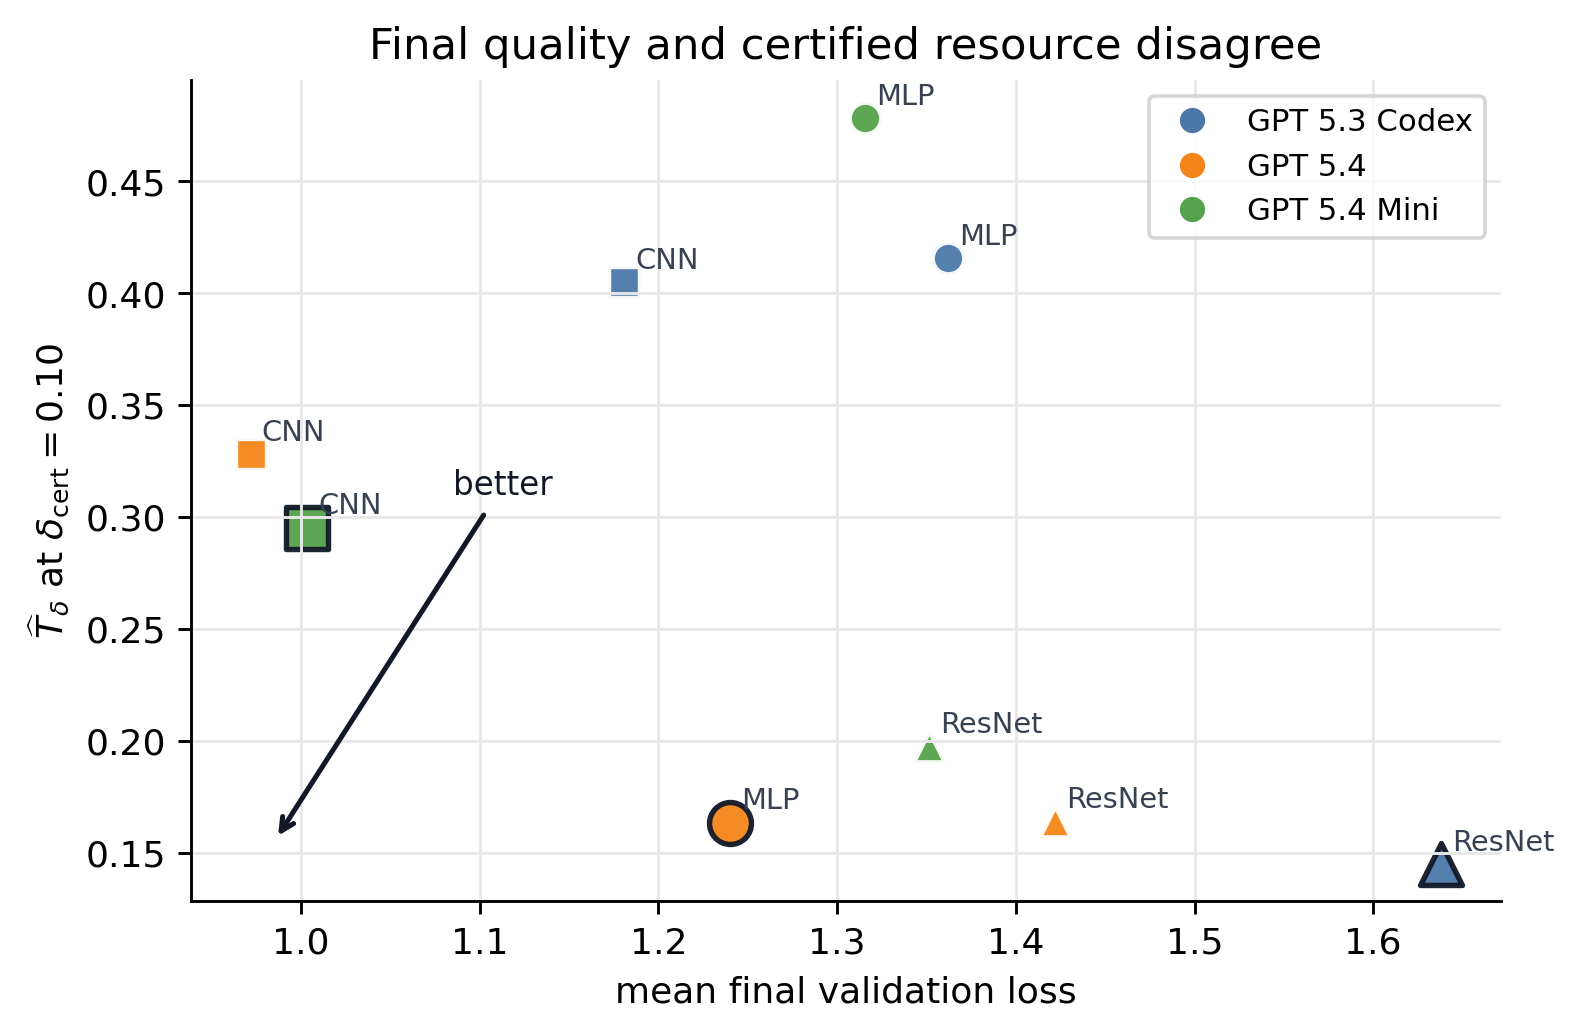
\includegraphics[width=0.86\linewidth]{figures/autoresearch/quality_vs_certified_resource.png}
\caption{Final validation loss versus empirical certified resource at \(\gamma=0.05\) and \(\delta_{\mathrm{cert}}=0.10\).
Points are mode--agent-system cells; larger outlined points are the mode-conditioned frontier from Table~\ref{tab:worker-frontier-accounting}.
The plot shows why final quality alone is not a sufficient deployment criterion.}
\label{fig:app-quality-resource-scatter}
\end{figure}

\begin{figure}[p]
\centering
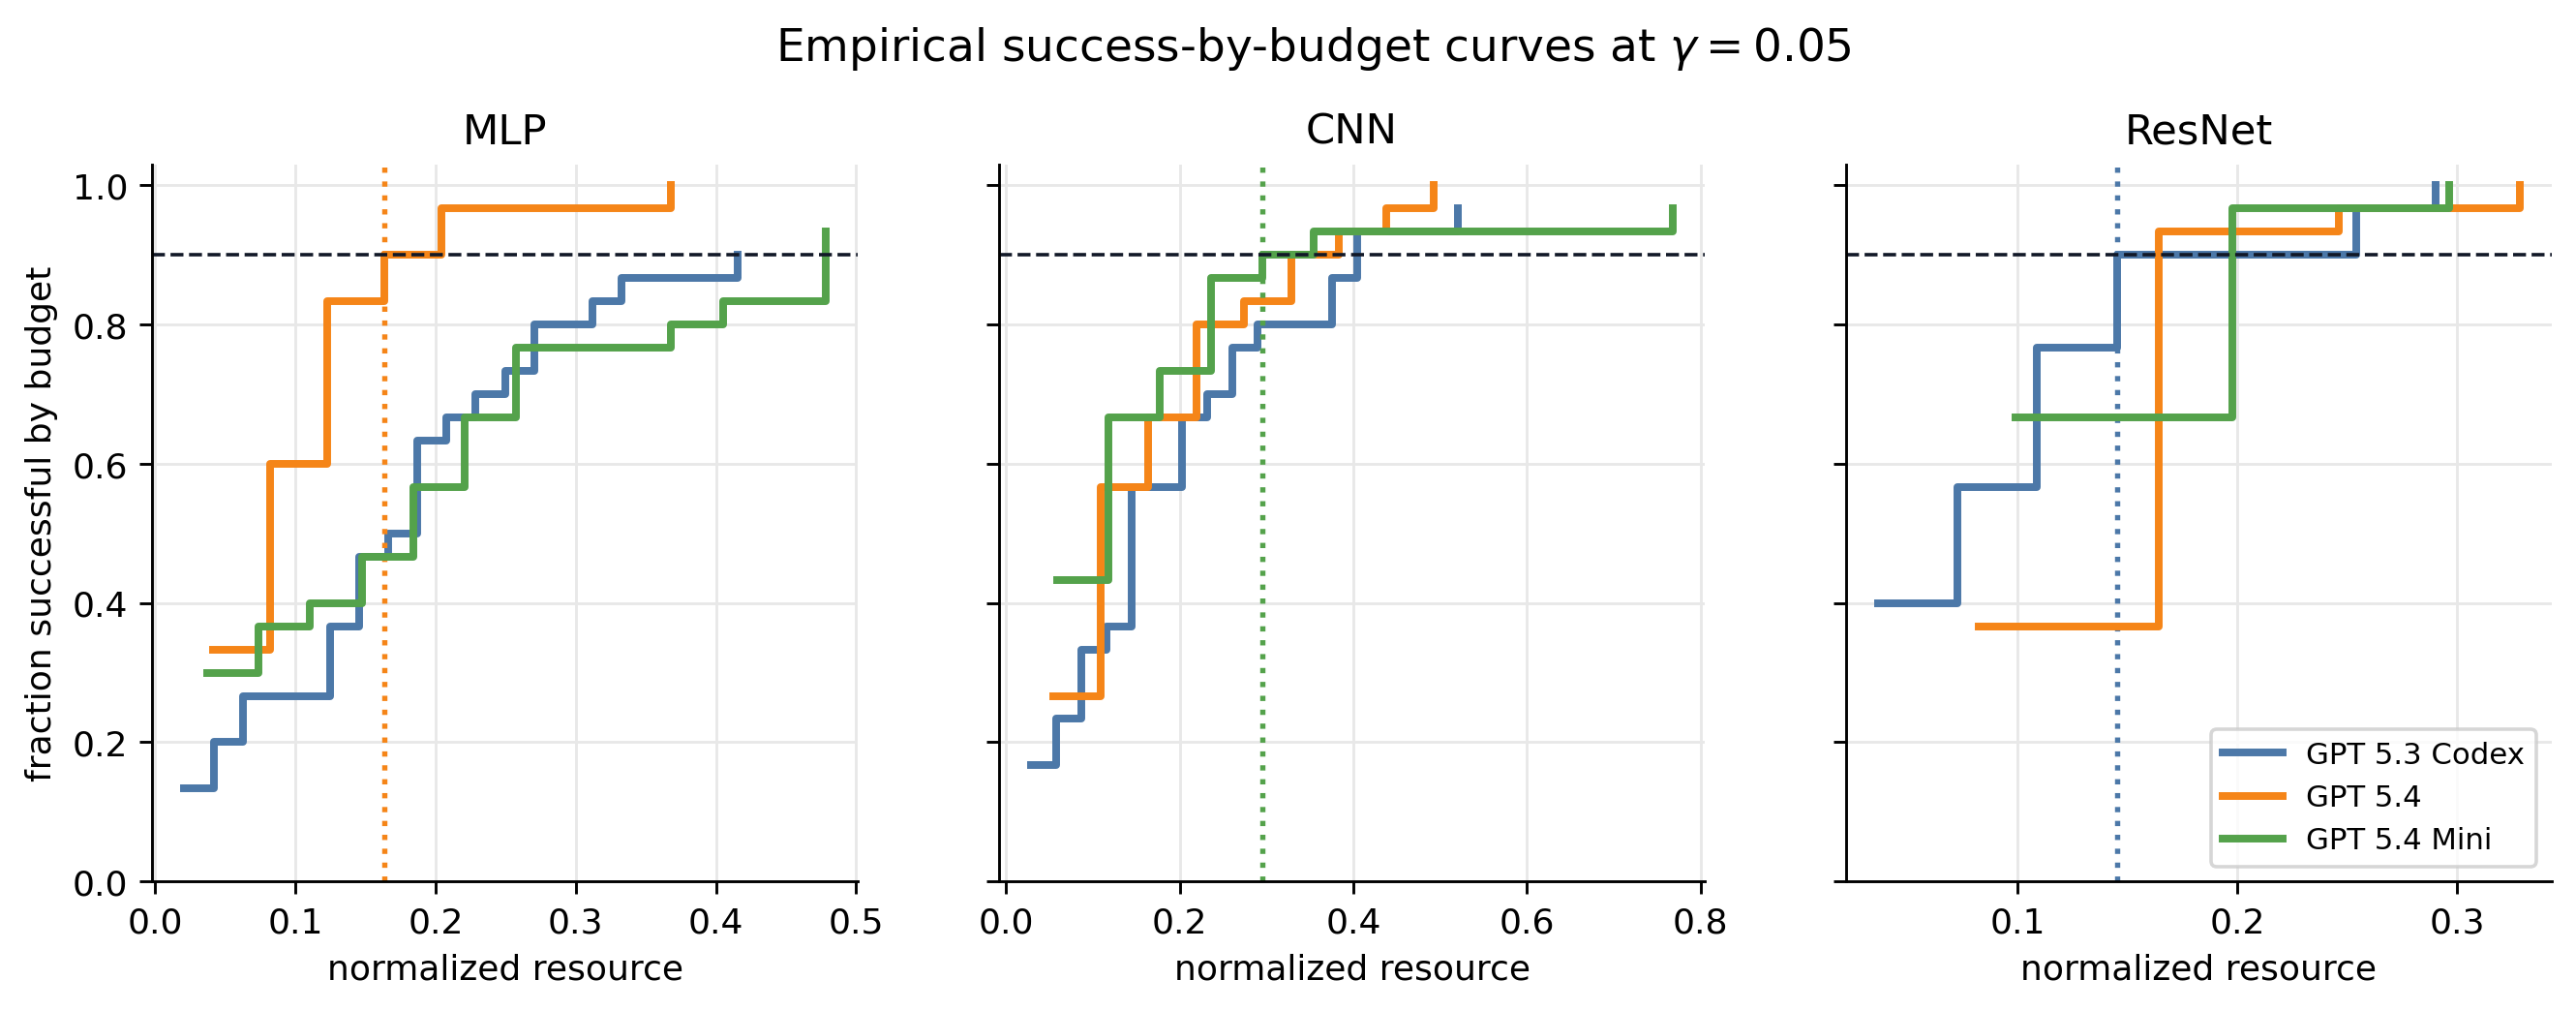
\includegraphics[width=\linewidth]{figures/autoresearch/first_hit_ecdf_by_mode.png}
\caption{Success-by-budget curves used to compute \(\widehat T_{\delta}\).
The dashed horizontal line marks \(90\%\) success, corresponding to \(\delta_{\mathrm{cert}}=0.10\).
Vertical dotted lines mark the mode-conditioned frontier value in each mode.}
\label{fig:app-first-hit-ecdf}
\end{figure}

\begin{figure}[p]
\centering
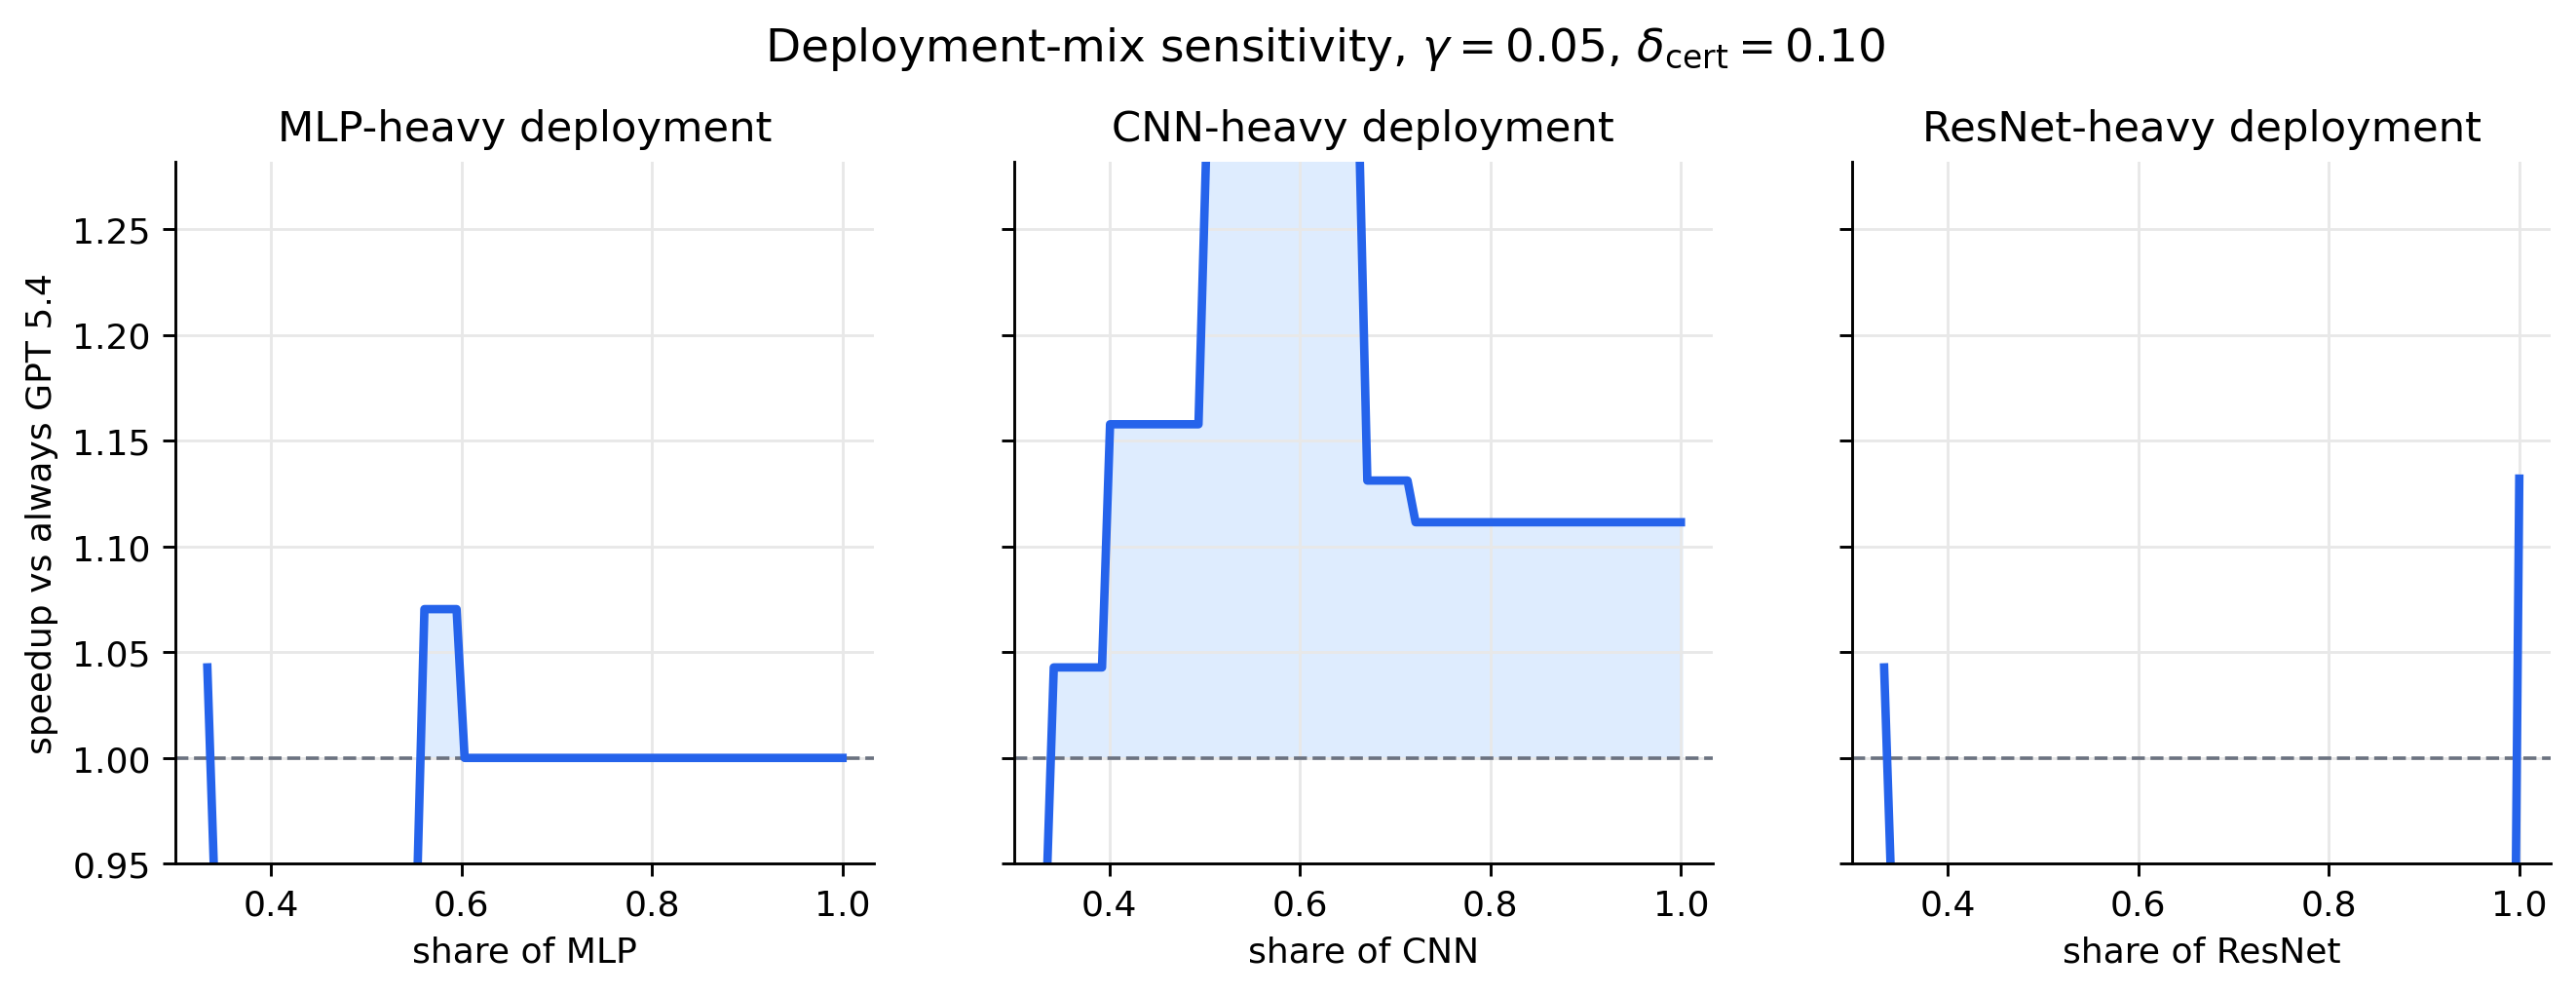
\includegraphics[width=\linewidth]{figures/autoresearch/deployment_mix_sensitivity.png}
\caption{Deployment-mix sensitivity for \(\gamma=0.05\) and \(\delta_{\mathrm{cert}}=0.10\).
Each panel increases the share of one mode while splitting the remaining mass equally across the other two.
The mode-conditioned policy remains above the no-speedup baseline across the displayed mixtures.}
\label{fig:app-deployment-mix-sensitivity}
\end{figure}

\begin{figure}[ht]
\centering
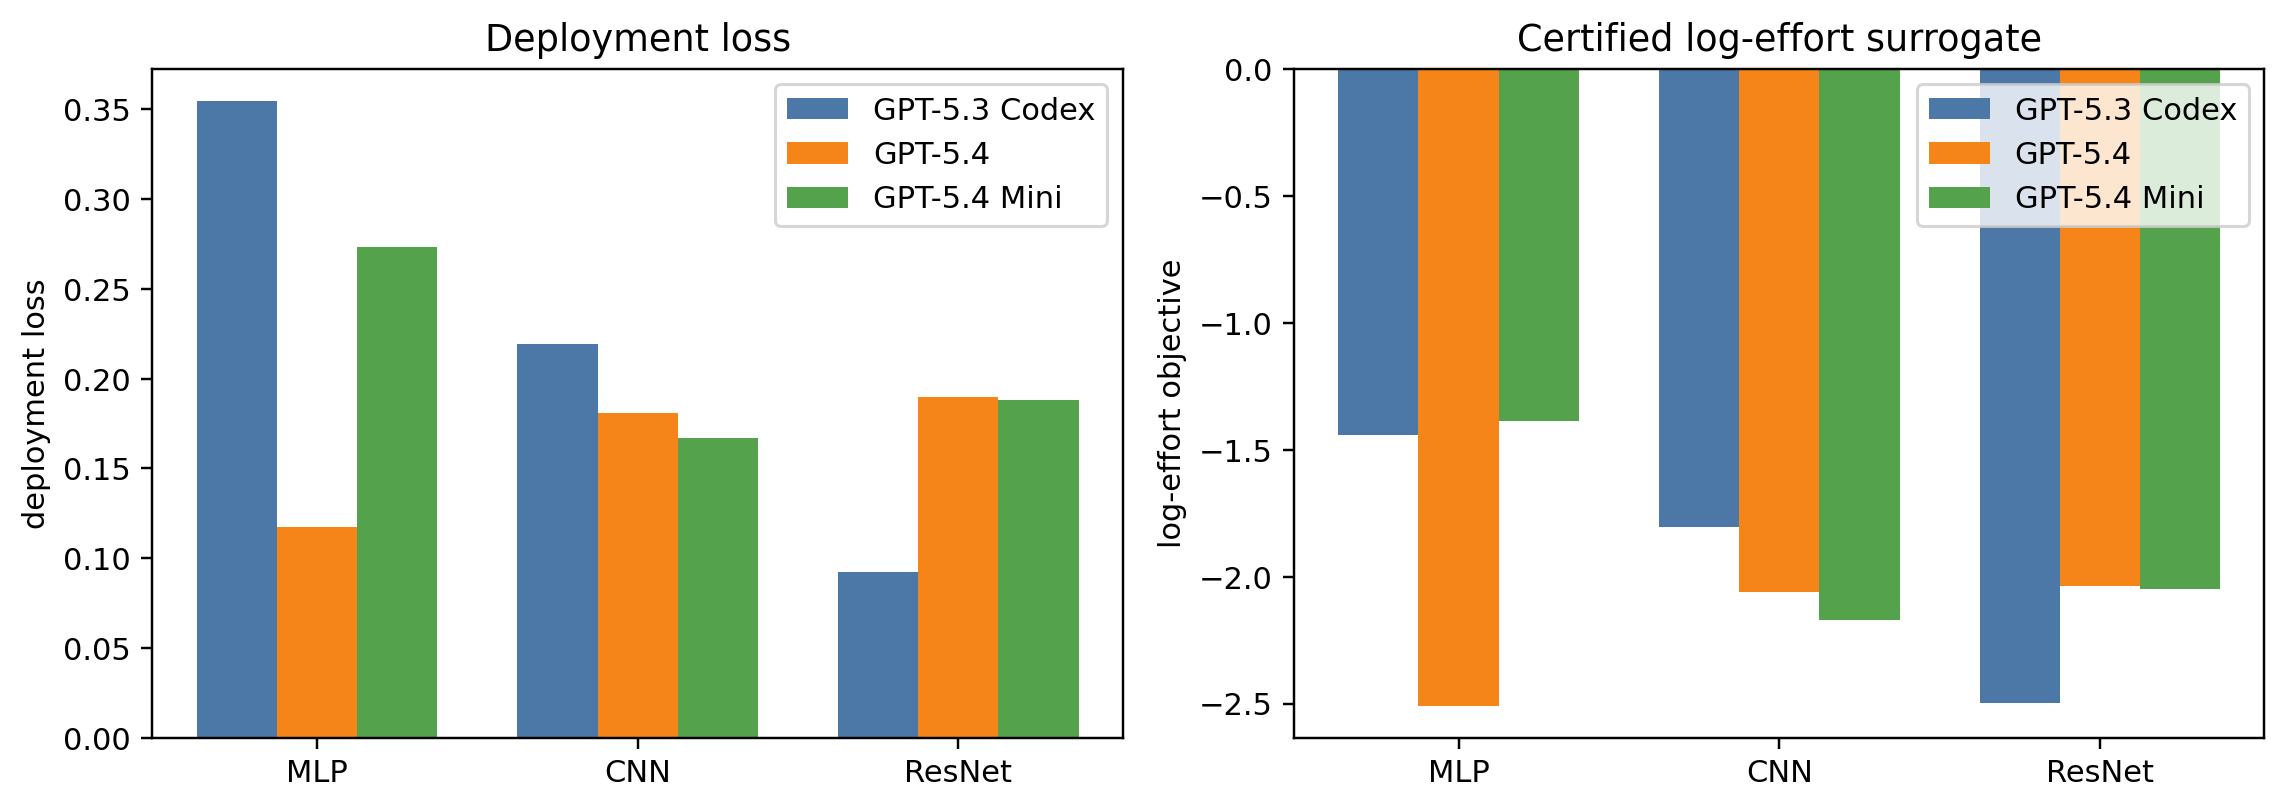
\includegraphics[width=\linewidth]{figures/autoresearch/threeworker_deployment_frontier.png}
\caption{Agent-system frontier visualization for the accounting quantities in Table~\ref{tab:worker-frontier-accounting}.
The plot is diagnostic only: the main text table reports the numerical terms used for the deployment recommendation.}
\label{fig:app-threeworker-frontier}
\end{figure}

\begin{figure}[ht]
\centering
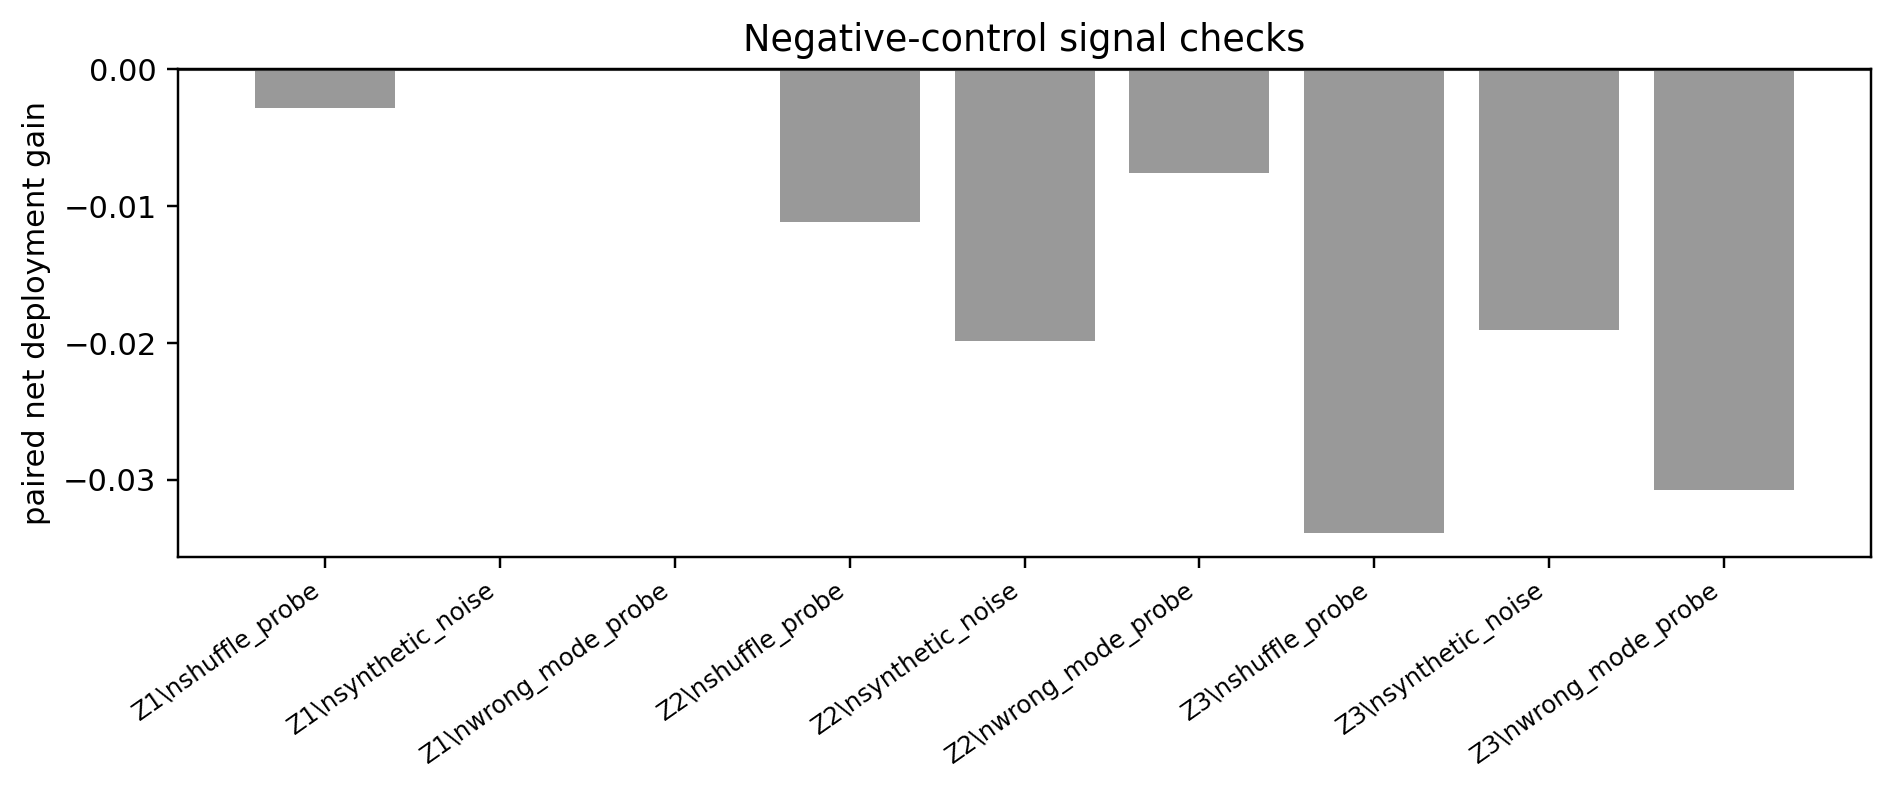
\includegraphics[width=\linewidth]{figures/autoresearch/threeworker_negative_controls.png}
\caption{Earlier probe-router negative-control audit for shuffled probes, wrong-mode probes, and synthetic noise records.
This diagnostic checks schema and context-burden artifacts for the probe-style router records; it is separate from the candidate-agent scout audit in Table~\ref{tab:candidate-scout-router}.}
\label{fig:app-negative-controls}
\end{figure}

\subsection{Pooled threshold and trajectory diagnostics}
\label{app:pilot-threshold-diagnostics}

\begin{figure}[p]
\centering
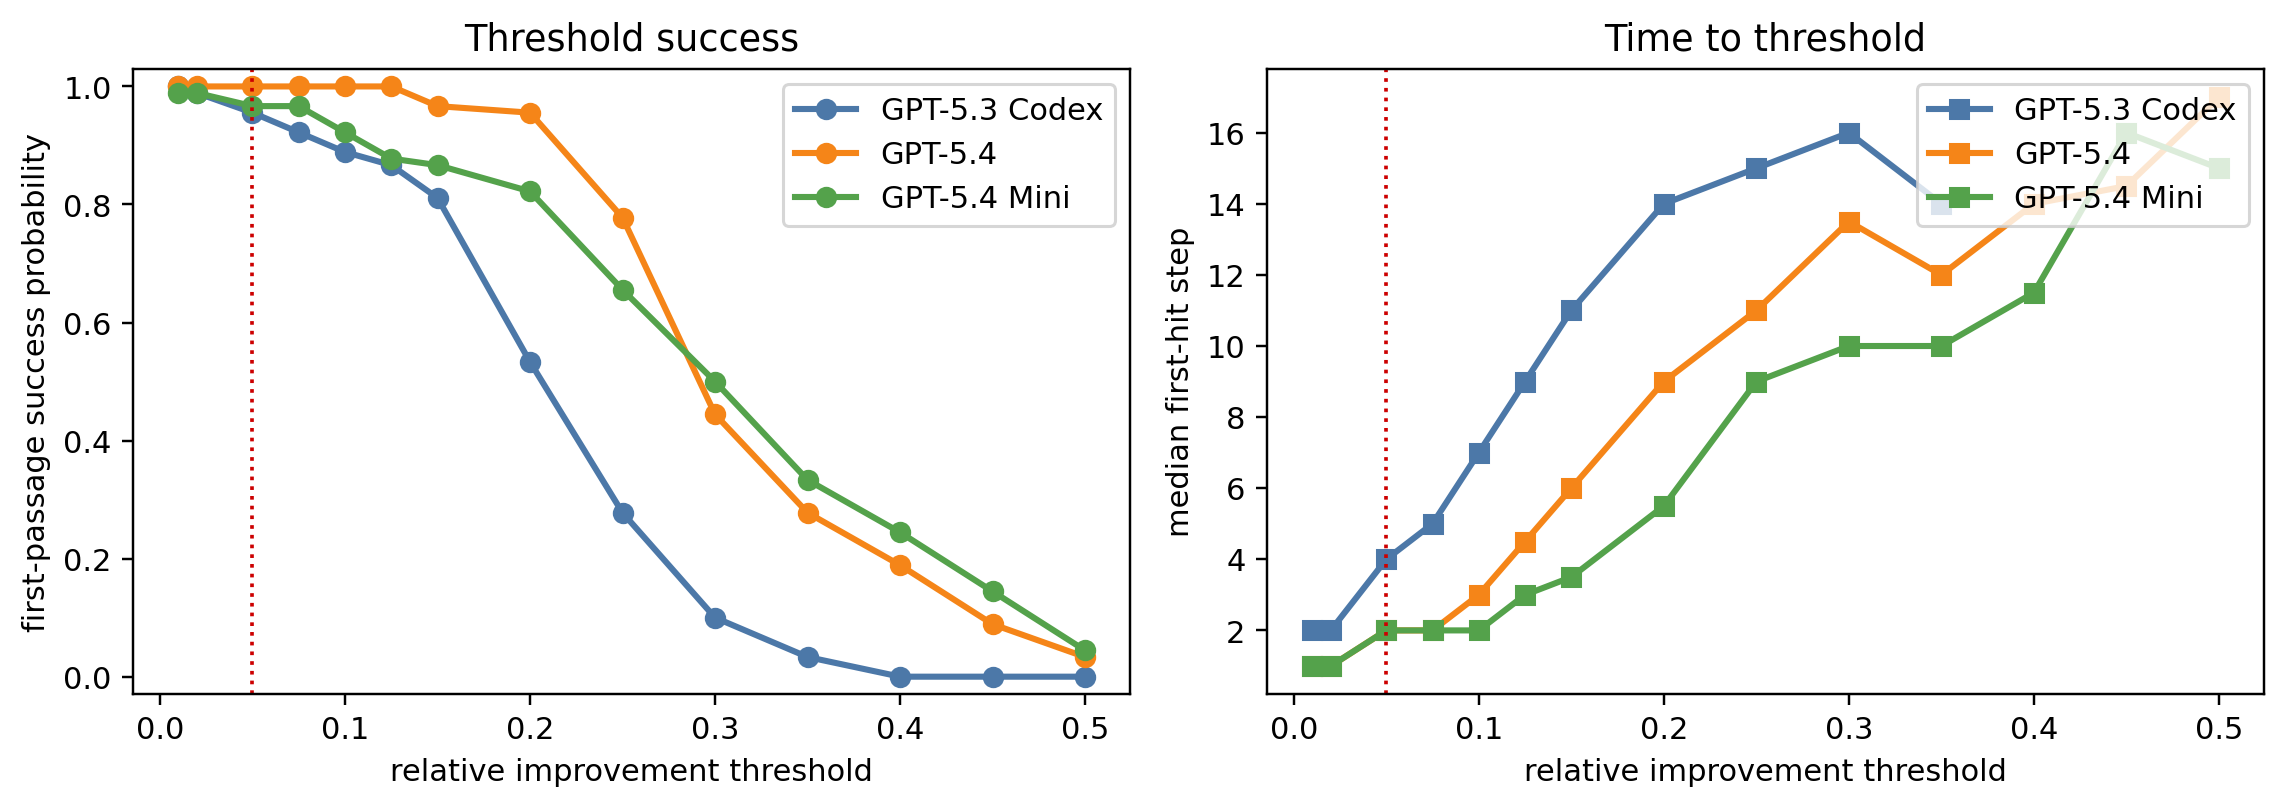
\includegraphics[width=\linewidth]{figures/autoresearch/threeworker_threshold_sensitivity.png}
\caption{Threshold sensitivity for the three-agent-system pooled panel.
The red line marks the operating threshold \(\gamma=0.05\).
At this threshold, entry success is near saturated while mean first-hit time remains low, which makes \(\gamma=0.05\) a pragmatic operating point for studying time-to-certified-solution.
The sharp drop at larger thresholds shows why the exact threshold is not an innocuous plotting choice.}
\label{fig:app-threshold-sensitivity-zoom}
\end{figure}

\begin{figure}[p]
\centering
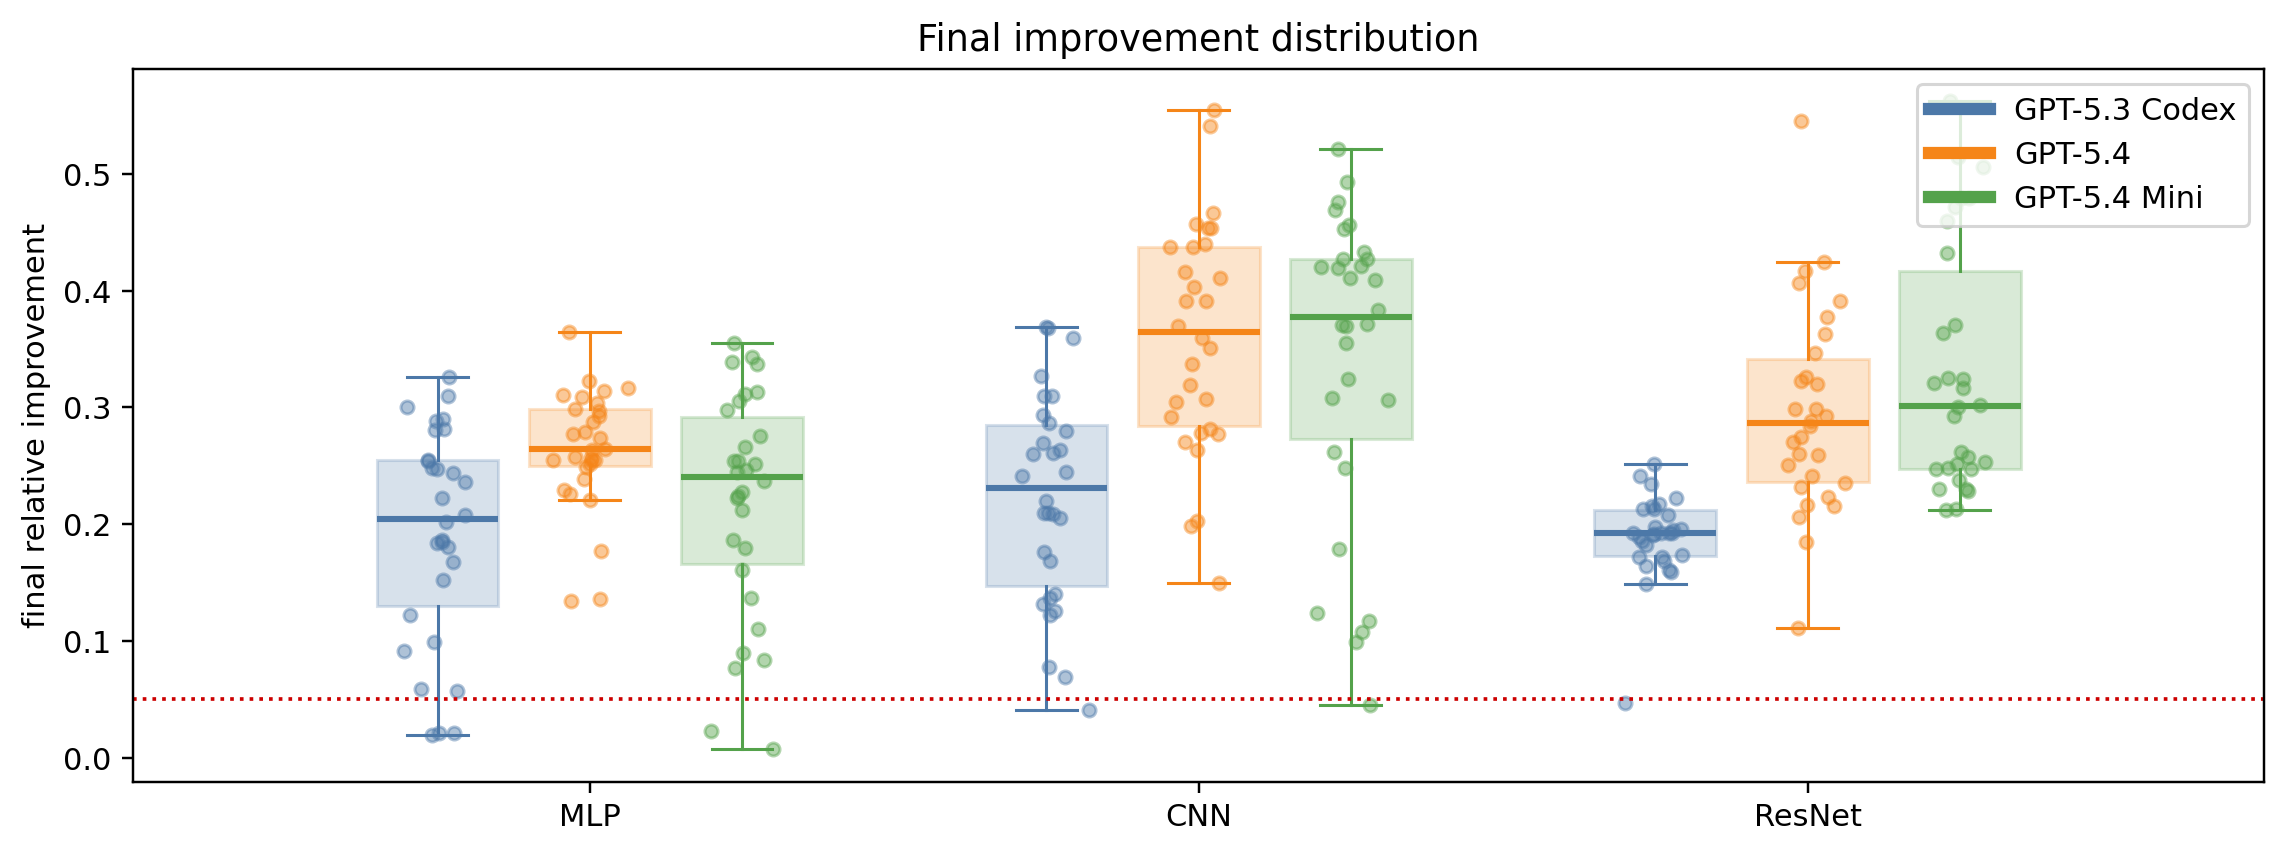
\includegraphics[width=\linewidth]{figures/autoresearch/threeworker_improvement_distribution.png}
\caption{Run-level improvement distribution for the three analyzed workers.
Dots show final best-visible relative improvement and thick ticks mark worker medians.
The survival plot makes the threshold choice explicit: near \(\delta=0.05\), most runs succeed, but the ordering and separation change at higher thresholds.
This diagnostic supports the paper's claim that final quality, first-passage success, and deployment loss are distinct empirical objects.}
\label{fig:app-improvement-distribution}
\end{figure}

\begin{figure}[p]
\centering
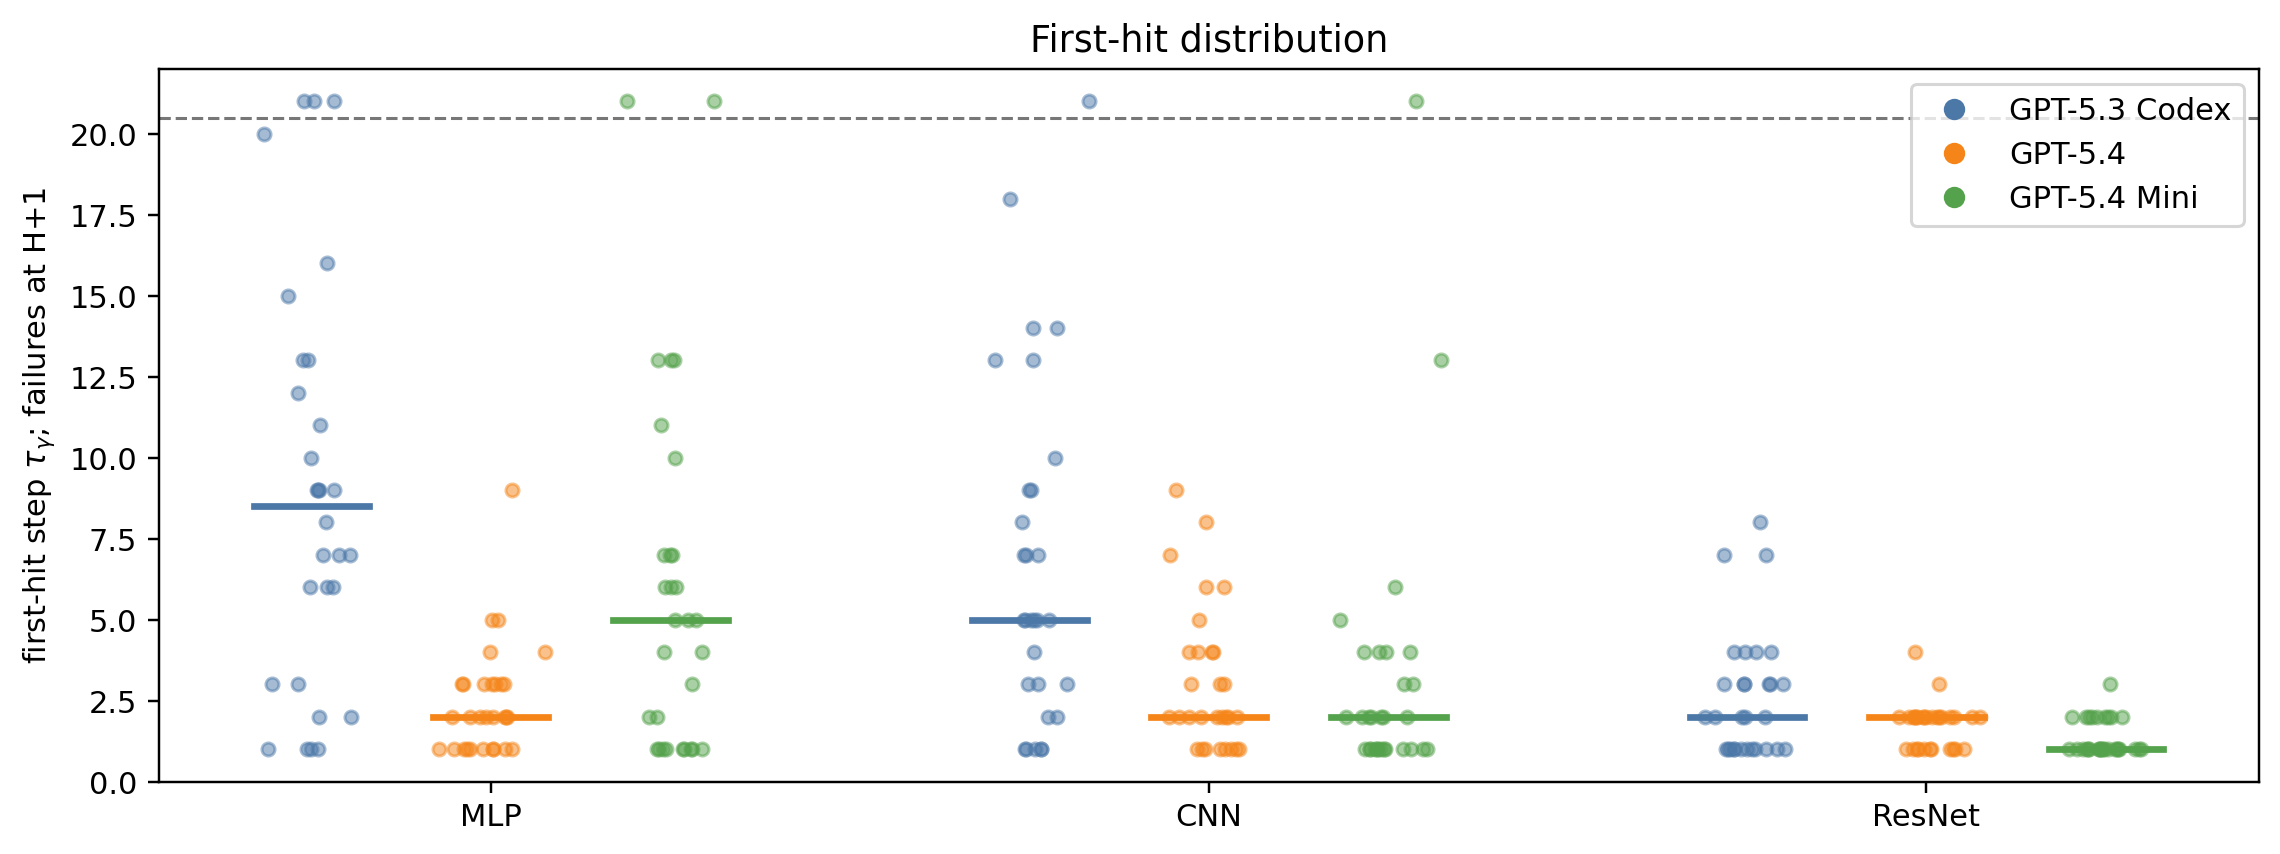
\includegraphics[width=\linewidth]{figures/autoresearch/threeworker_tau_distribution.png}
\caption{Pooled time-to-success distribution by task mode and worker.
The scatter plots expose mode-conditional heterogeneity: Mini is fastest on \textit{compact CNN} and \textit{micro ResNet}, while \texttt{gpt\_5\_4} is fastest on \textit{MLP-flat}.
This is the empirical object behind the cost and competence terms of the four-term decomposition.}
\label{fig:app-tau-distribution}
\end{figure}

\begin{figure}[p]
\centering
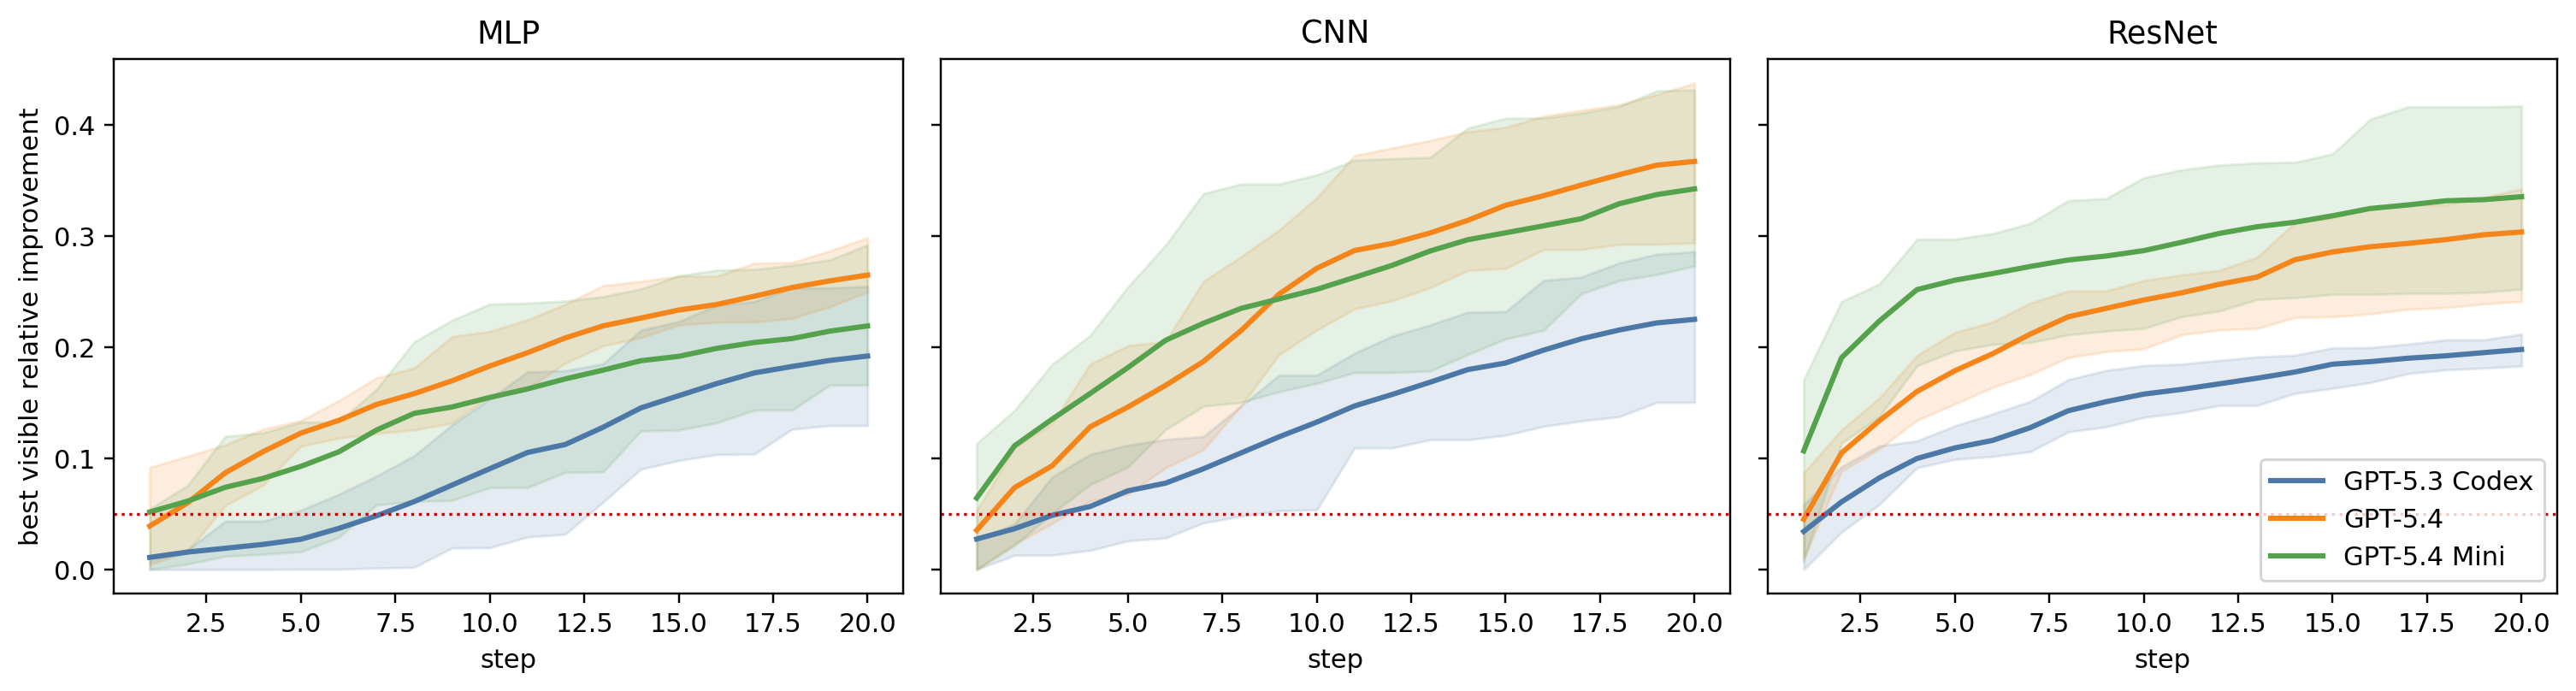
\includegraphics[width=\linewidth]{figures/autoresearch/threeworker_relative_improvement_trajectories.png}
\caption{Best-so-far improvement trajectories.
The mean trajectories show that early progress and final quality vary by mode and worker, but the deployment accounting in the main text shows that this does not automatically imply lower deployment loss after cost is charged.
This contrast is the main empirical reason to separate worker competence from deployment value.}
\label{fig:app-improvement-trajectories}
\end{figure}

\subsection{Pooled cost diagnostics}
\label{app:pilot-cost-diagnostics}

\begin{figure}[p]
\centering
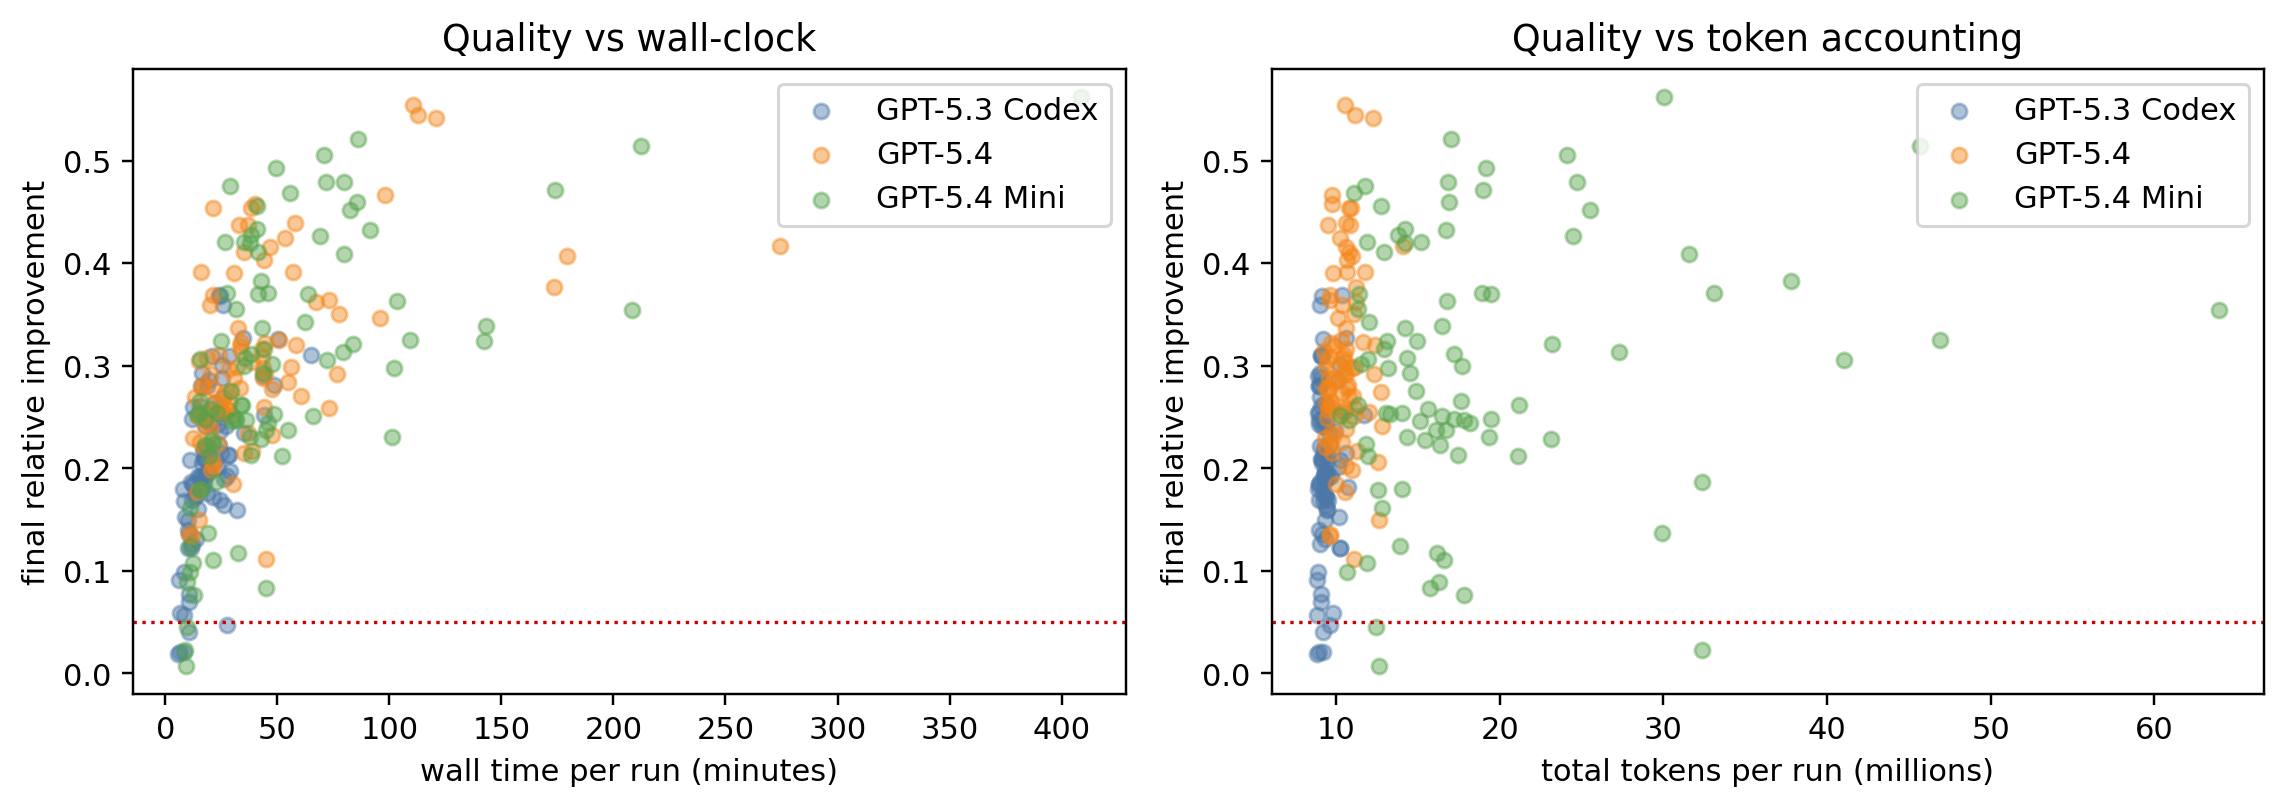
\includegraphics[width=\linewidth]{figures/autoresearch/threeworker_worker_cost_quality_diagnostics.png}
\caption{Worker cost--quality diagnostics.
Each point is a valid pooled run.
The plots show that better final improvement is accompanied by substantial variation in wall-clock time, total token accounting, and generated-token volume.
This supports the paper's budget-aware framing: worker choice cannot be reduced to final improvement alone.}
\label{fig:app-worker-cost-quality-full}
\end{figure}

\begin{figure}[p]
\centering
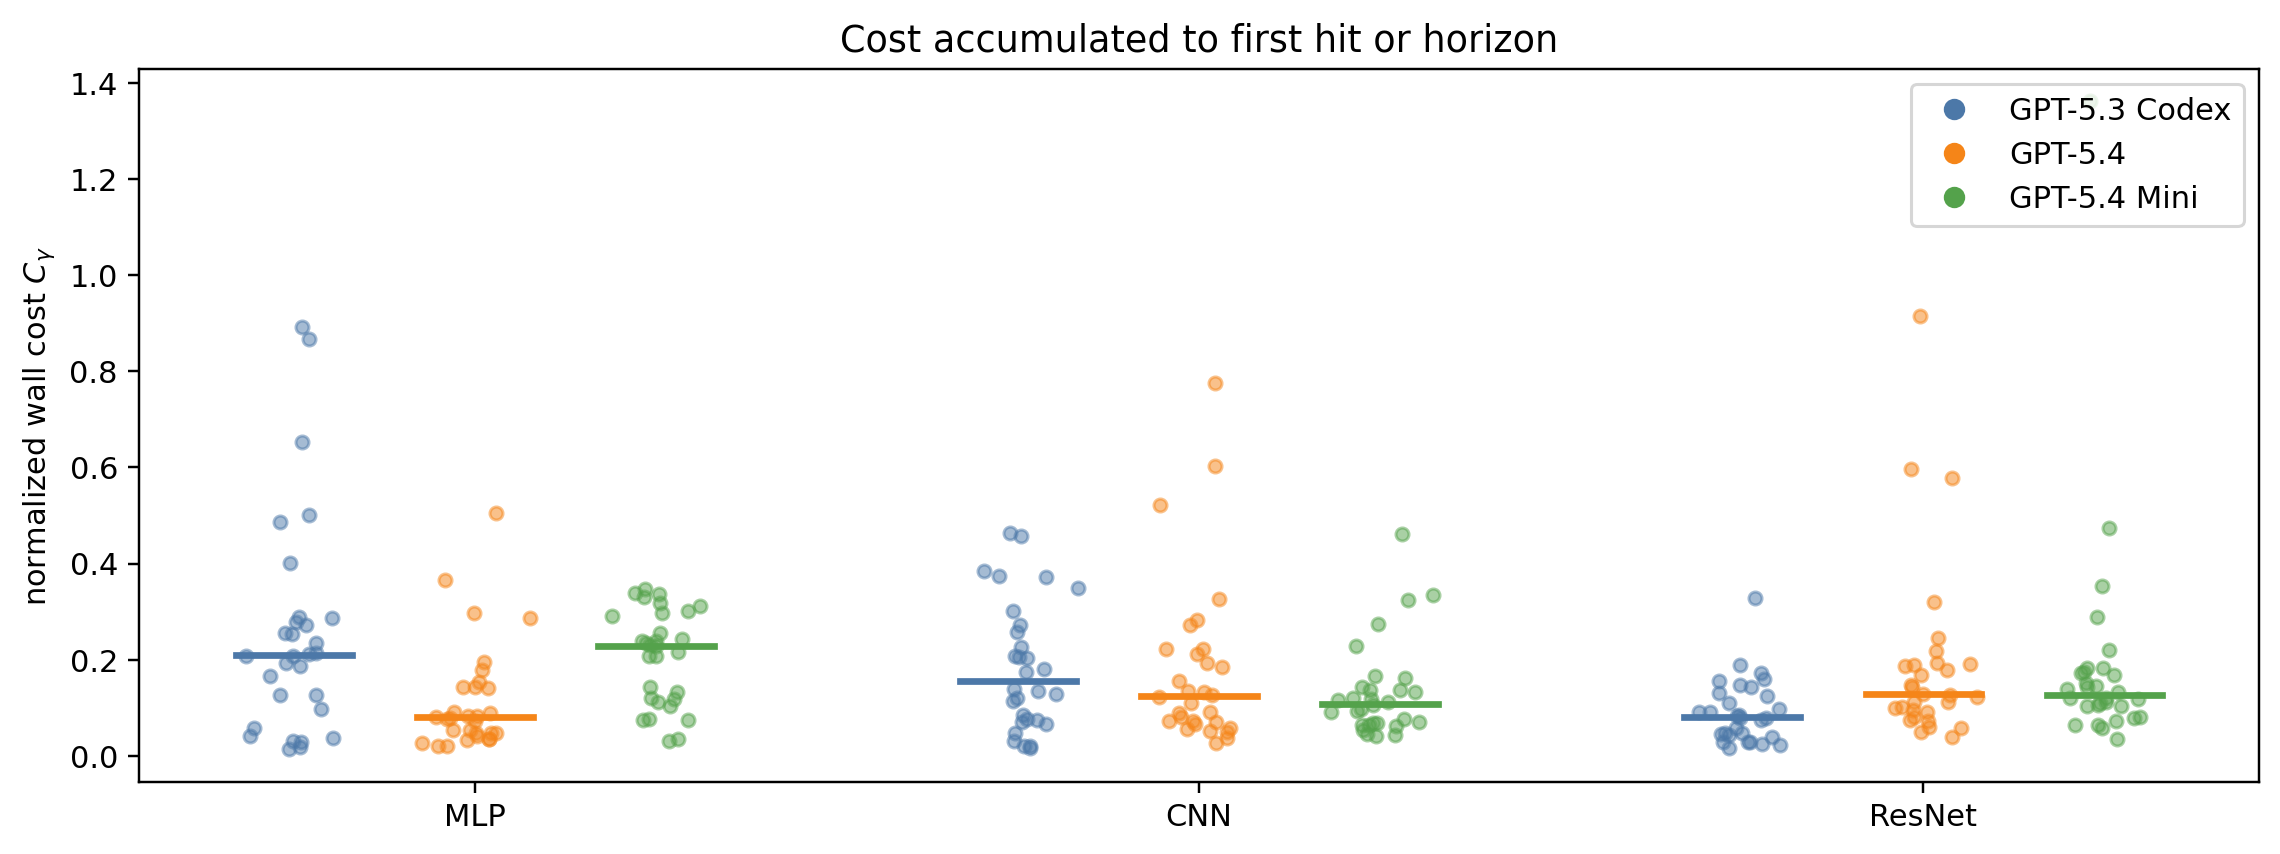
\includegraphics[width=\linewidth]{figures/autoresearch/threeworker_cost_to_tau_by_mode_worker.png}
\caption{Resource cost accumulated to first hit or horizon.
Mode-conditional cost spreads are large, which is why the retry-crossover theorem is treated as a cost-sensitive design rule rather than a generic endorsement of weaker workers.}
\label{fig:app-cost-to-tau-full}
\end{figure}

\begin{figure}[p]
\centering
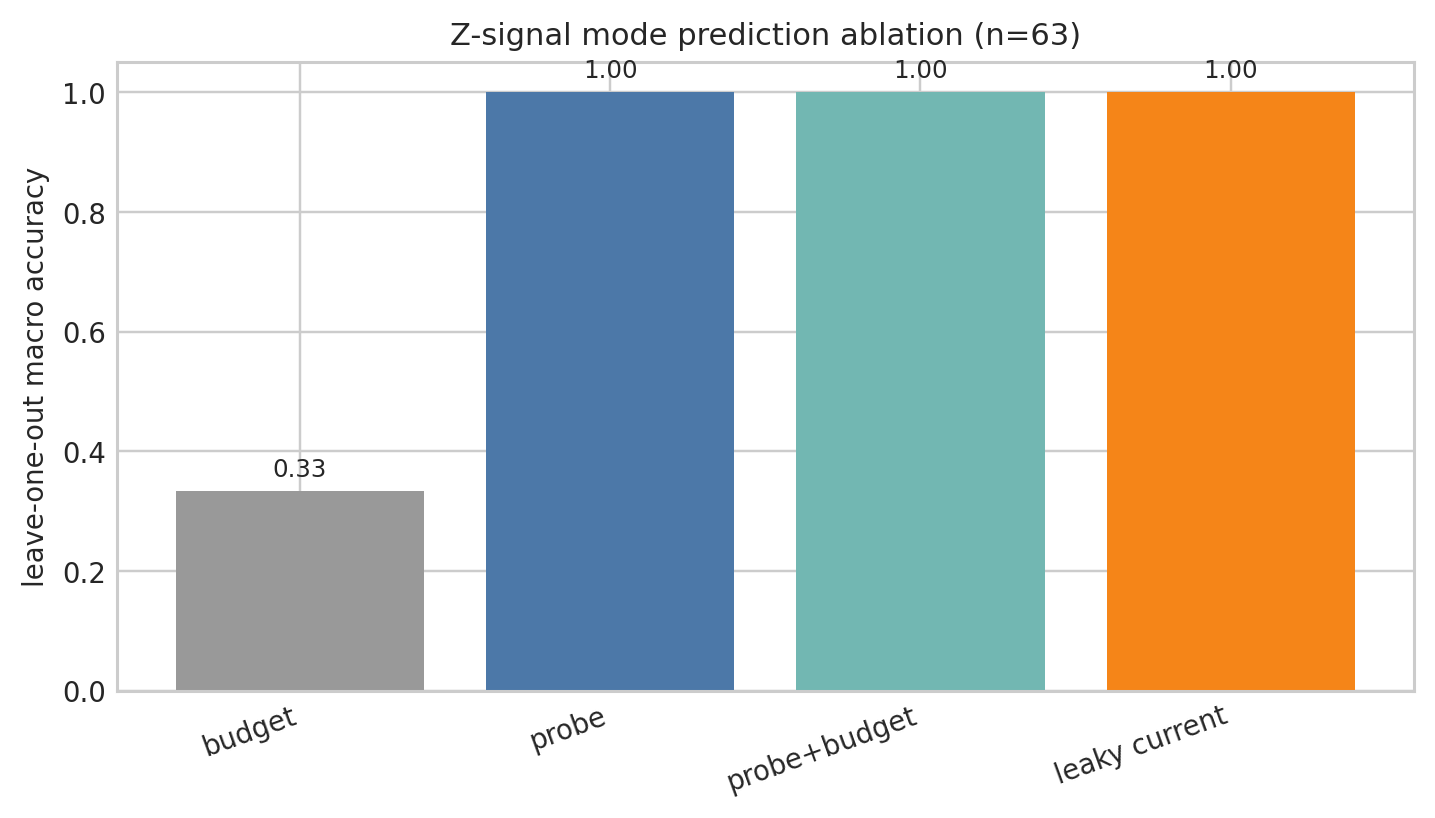
\includegraphics[width=0.92\linewidth]{figures/autoresearch/diag_z_signal_ablation.png}
\caption{Router-facing signal ablation.
The diagnostic tests whether progressively richer records expose the task-mode structure used in the accounting analysis.}
\label{fig:app-router}
\end{figure}

\clearpage
\section*{NeurIPS Paper Checklist}


\begin{enumerate}

\item {\bf Claims}
    \item[] Question: Do the main claims made in the abstract and introduction accurately reflect the paper's contributions and scope?
    \item[] Answer: \answerYes{}
    \item[] Justification: The abstract and introduction state the paper's scope: verifiable agentic systems, a packed latent-mode assumption, decomposition-guided selection, and a controlled fixed-prototype experimental protocol. The discussion section separates theory-facing and deployment-facing claims.
\item {\bf Limitations}
    \item[] Question: Does the paper discuss the limitations of the work performed by the authors?
    \item[] Answer: \answerYes{}
    \item[] Justification: Section~\ref{sec:discussion} discusses the packed-mode assumption, small live-agent sample sizes, finite design menus, oracle mode labels, and current cost-measurement limitations.
\item {\bf Theory assumptions and proofs}
    \item[] Question: For each theoretical result, does the paper provide the full set of assumptions and a complete (and correct) proof?
    \item[] Answer: \answerYes{}
    \item[] Justification: Assumption~\ref{ass:packed} states the assumptions for the main theoretical result, Theorem~\ref{thm:four-term} includes a proof sketch, and Appendix~\ref{app:proofs} gives the algebraic proof and pilot concentration details.
    \item {\bf Experimental result reproducibility}
    \item[] Question: Does the paper fully disclose all the information needed to reproduce the main experimental results of the paper to the extent that it affects the main claims and/or conclusions of the paper (regardless of whether the code and data are provided or not)?
    \item[] Answer: \answerYes{}
    \item[] Justification: Section~\ref{sec:experiments} describes the AutoResearch task instantiation, task modes, model menu, router-visible signals, horizons, metrics, and evaluation protocol; Appendix~\ref{app:experiment-details} specifies the required logs, estimators, and run-metadata fields.

\item {\bf Open access to data and code}
    \item[] Question: Does the paper provide open access to the data and code, with sufficient instructions to faithfully reproduce the main experimental results, as described in supplemental material?
    \item[] Answer: \answerNo{}
    \item[] Justification: The paper is written against an existing repository and includes reproducibility commands, but an anonymized public code/data release is not included in the current submission package.

\item {\bf Experimental setting/details}
    \item[] Question: Does the paper specify all the training and test details (e.g., data splits, hyperparameters, how they were chosen, type of optimizer) necessary to understand the results?
    \item[] Answer: \answerYes{}
    \item[] Justification: Section~\ref{sec:experiments} describes the AutoResearch task instantiation, task modes, model menu, router-visible signals, primary estimators, horizons, and evaluation design. Additional implementation details are listed in Appendix~\ref{app:experiment-details}.
\item {\bf Experiment statistical significance}
    \item[] Question: Does the paper report error bars suitably and correctly defined or other appropriate information about the statistical significance of the experiments?
    \item[] Answer: \answerYes{}
    \item[] Justification: Section~\ref{sec:experiments} and Appendix~\ref{app:experiment-details} specify Wilson intervals, bootstrap intervals, survival curves, calibration diagnostics, and held-out evaluation for the reported protocol.
\item {\bf Experiments compute resources}
    \item[] Question: For each experiment, does the paper provide sufficient information on the computer resources (type of compute workers, memory, time of execution) needed to reproduce the experiments?
    \item[] Answer: \answerNo{}
    \item[] Justification: The paper reports wall-clock costs and run counts but does not provide a complete compute-resource table for every experiment.
\item {\bf Code of ethics}
    \item[] Question: Does the research conducted in the paper conform, in every respect, with the NeurIPS Code of Ethics \url{https://neurips.cc/public/EthicsGuidelines}?
    \item[] Answer: \answerYes{}
    \item[] Justification: The work studies verifiable benchmark tasks and does not involve human subjects, sensitive personal data, or released high-risk models. The submission preserves anonymity and follows NeurIPS code and data policies.

\item {\bf Broader impacts}
    \item[] Question: Does the paper discuss both potential positive societal impacts and negative societal impacts of the work performed?
    \item[] Answer: \answerYes{}
    \item[] Justification: Section~\ref{sec:discussion} notes positive uses in cost-aware and transparent agent deployment as well as limitations and failure modes. The work is methodological and does not introduce a new generative model or dataset of people.
\item {\bf Safeguards}
    \item[] Question: Does the paper describe safeguards that have been put in place for responsible release of data or models that have a high risk for misuse (e.g., pre-trained language models, image generators, or scraped datasets)?
    \item[] Answer: \answerNA{}
    \item[] Justification: The paper does not release a pre-trained model, image generator, scraped dataset, or other asset with high misuse risk. It evaluates agent harnesses on synthetic or generated benchmark tasks.
\item {\bf Licenses for existing assets}
    \item[] Question: Are the creators or original owners of assets (e.g., code, data, models), used in the paper, properly credited and are the license and terms of use explicitly mentioned and properly respected?
    \item[] Answer: \answerYes{}
    \item[] Justification: The related-work section cites existing papers and systems used for positioning, and the experimental section describes the benchmark surfaces. Released code and benchmark assets include explicit license details.
\item {\bf New assets}
    \item[] Question: Are new assets introduced in the paper well documented and is the documentation provided alongside the assets?
    \item[] Answer: \answerYes{}
    \item[] Justification: The work introduces a code harness and analysis artifacts as research assets, and Appendix~\ref{app:experiment-details} documents the required logging and configuration fields.
\item {\bf Crowdsourcing and research with human subjects}
    \item[] Question: For crowdsourcing experiments and research with human subjects, does the paper include the full text of instructions given to participants and screenshots, if applicable, as well as details about compensation (if any)?
    \item[] Answer: \answerNA{}
    \item[] Justification: The paper does not involve crowdsourcing or research with human subjects.
\item {\bf Institutional review board (IRB) approvals or equivalent for research with human subjects}
    \item[] Question: Does the paper describe potential risks incurred by study participants, whether such risks were disclosed to the subjects, and whether Institutional Review Board (IRB) approvals (or an equivalent approval/review based on the requirements of your country or institution) were obtained?
    \item[] Answer: \answerNA{}
    \item[] Justification: The paper does not involve crowdsourcing or research with human subjects, so IRB or equivalent approval is not applicable.
\item {\bf Declaration of LLM usage}
    \item[] Question: Does the paper describe the usage of LLMs if it is an important, original, or non-standard component of the core methods in this research? Note that if the LLM is used only for writing, editing, or formatting purposes and does \emph{not} impact the core methodology, scientific rigor, or originality of the research, declaration is not required.
    %this research?
    \item[] Answer: \answerYes{}
    \item[] Justification: LLMs are central to the evaluated agent designs. Section~\ref{sec:experiments} describes the three-worker menu, fixed prompt-only router, sequential signal protocol, model-identifier logging, and routing-output requirements.
\end{enumerate}


\end{document}
